\documentclass[a4paper]{report}
\usepackage{amsmath, amscd, amssymb, amsthm, latexsym}
\usepackage[spanish]{babel}
\usepackage{enumerate}
\usepackage{float}
\usepackage[table]{xcolor}
\usepackage{geometry}
\usepackage{url}
\usepackage{booktabs}
\usepackage{tabularx}
\usepackage{graphicx}
\usepackage{caption}
\usepackage{hyperref}
\usepackage{graphics}
\usepackage{tikz}
\usepackage{multirow}
\usepackage{clrscode3e}
\usepackage{environ}
\usepackage[skip=10pt,indent=20pt]{parskip}


\graphicspath{{img/}}

\hypersetup{
    colorlinks=true,%
    linkcolor=blue!80!red,%
    urlcolor=green!70!black
}

\captionsetup[figure]{%
    font=small,%
    justification=centering,%
    width=0.6\textwidth
}

% Comandos caseros
\newcommand{\BigO}[1]{\ensuremath{\mathcal{O}(#1)}}
\newcommand{\BigOmega}[1]{\ensuremath{\Omega(#1)}}
\newcommand{\BigTheta}[1]{\ensuremath{\Theta(#1)}}

\newcommand{\code}{\texttt}

\newcommand{\si}{\text{si }}
\newcommand{\ecc}{\text{en caso contrario}}

\newcommand{\N}{\mathbb{N}}
\newcommand{\Z}{\mathbb{Z}}
\newcommand{\R}{\mathbb{R}}

\newcommand{\Each}{\kw{each}\ }

\fboxsep=10pt
\NewEnviron{problema}{%
\medskip
\begin{center}
    \fbox{%
        \begin{minipage}{32em}
            \textbf{Problema:}
            \smallskip
            
            \BODY
        \end{minipage}
    }
\end{center}
\medskip
}


\newtheorem*{theorem*}{Teorema}
\newtheorem*{lemma*}{Lema}

\title{%
    Resumen para Algoritmos y Estructuras de Datos III\\
    \small Basado en \href{https://campus.exactas.uba.ar/pluginfile.php/390238/mod_resource/content/1/resumen.pdf}{esta guía de estudio}.%
}
\author{Tomás Spognardi}
\date{\today}

\begin{document}

\maketitle



\tableofcontents

\input{chapters/1-tecnicas-de-diseño.tex}

\chapter{Introducción a Teoría de Grafos}

\section{Grafos}

\subsection{Definición}

Un \textit{grafo} es un par ordenado $G = (V, E)$: el conjunto $V$, de \textit{vértices} o \textit{nodos} , y el de aristas/arcos $E$, que relacionan a esos nodos.

En el caso de los grafos \textit{no dirigidos} (o simplemente grafos), $E \subseteq \{\{v_1, v_2\}\ |\ v_1,v_2 \in V, v_1 \neq v_2 \}$ es un conjunto de pares no ordenados de los elementos de $V$, conocidos como \textit{aristas}. Por otro lado, para los \textit{grafos dirigidos} (también llamados \textit{digrafos}), $E \subseteq V \times V$ tiene pares ordenados de nodos, y sus elementos se denominan arcos. Se suele realizar un abuso de notación menor, utilizando $(v, w)$ para referirse tanto a aristas como arcos.

\begin{figure}[H]
    \centering
    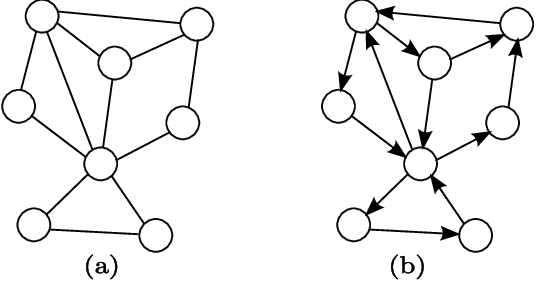
\includegraphics[width=0.5\textwidth]{ejemplo_grafo.png}
    \small
    \caption*{Representaciones gráficas de un grafo (a) y un digrafo (b). Los círculos son los vértices, y las líneas/flechas son las aristas/arcos.}
\end{figure}

En general, se denota $n_G = |V|$ y $m_G = |E|$ para referirse a las cantidades de vértices y aristas. Cuando el grafo referido es inambigüo, se omite el subíndice\footnote{Lo mismo vale para el resto de las definiciones en esta sección.}.

\subsection{Vecinos}

Dados $v,w \in V$, se denominan \textit{adyacentes} cuando $e = (v,w) \in E$, y que $e$ es \textit{incidente} a $v$ y $w$. Similarmente, la \textit{vecindad} de $v$, denotada por $N_G(v)$ es el conjunto de vértices adyacentes a $v$, es decir:
$$N_G(v) = \{w \in V \mid (v, w) \in E\}$$

Por otro lado, la cantidad de aristas incidentes a un vértice $v$ se llama \textit{grado}, definida como:
$$d_G(v) = |N_G(v)|$$

\begin{theorem*}
    Dado un grafo de $G = (V, E)$, la suma de los grados de sus vértices es el doble de la cantidad de aristas. Es decir,
    $$\sum_{v \in V} d(v) = 2m$$
\end{theorem*}
\begin{proof}
    Se puede demostrar por inducción en $m$, la cantidad de aristas.

    \textbf{Caso base:} Se puede tomar como caso base $m = 0$. En un grafo sin aristas, todos los vértices tienen grado $0$, y por ende:
    $$\sum_{v \in V} d(v) = 0 = 2m$$

    \textbf{Paso inductivo:} Asumiendo que la propiedad se cumple para $m = k$, tomemos un grafo cualquiera $G = (V, E)$ con $|E| = k + 1$ aristas. Se puede elegir una arista cualquiera $e = (v, w) \in E$, y construir el grafo $G' = (V, E - {e})$ que resulta de quitar una de sus aristas. Como $m_{G'} = k$, se cumple la hipótesis inductiva:
    $$\sum_{u \in V} d_{G'}(u) = 2m_{G'} = 2k$$

    Luego, para el grafo original $G$, la adición de la arista $e$ solo incrementea el grado de los vértices $v$ y $w$. Concretamente:
    $$
        d_G(u) =
        \begin{cases}
            d_{G'}(u) + 1 & \si u = v \lor u = w \\
            d_{G'}(u)     & \ecc
        \end{cases}
    $$
    Por lo tanto, se tiene:
    \begin{align*}
        \sum_{u \in V} d_G(u) & = \sum_{v \in V - \{v, w\}} d_{G'}(u) + (d_{G'}(v) + 1) + (d_{G'}(w) + 1) \\
                              & = \sum_{u \in V} d_{G'}(u) + 2 \stackrel{HI}{=} 2k + 2 = 2(k + 1) = 2m_G
    \end{align*}

    Lo cual, por inducción, implica que la propiedad vale para todo $m \in \N$.

\end{proof}

\subsubsection{Complemento}

Dado un grafo $G = (V, E)$, su \textit{grafo complemento}, denotado como $\bar{G} = (V, \bar{E})$, tiene el mismo conjunto de vértices, pero cada par de vértices es adyacente en $\bar{G}$ si y solo si no lo es en $G$. Es decir,
$$\bar{E} = (V \times V) - E$$

\subsubsection{Grafos Completos}

El grafo $K_n$ es el \textit{grafo completo} de $n$ vértices, los cuales son todos adyacentes entre sí. Este grafo tiene $m_{K_n} = \frac{n(n-1)}{2}$.

\begin{figure}[H]
    \centering
    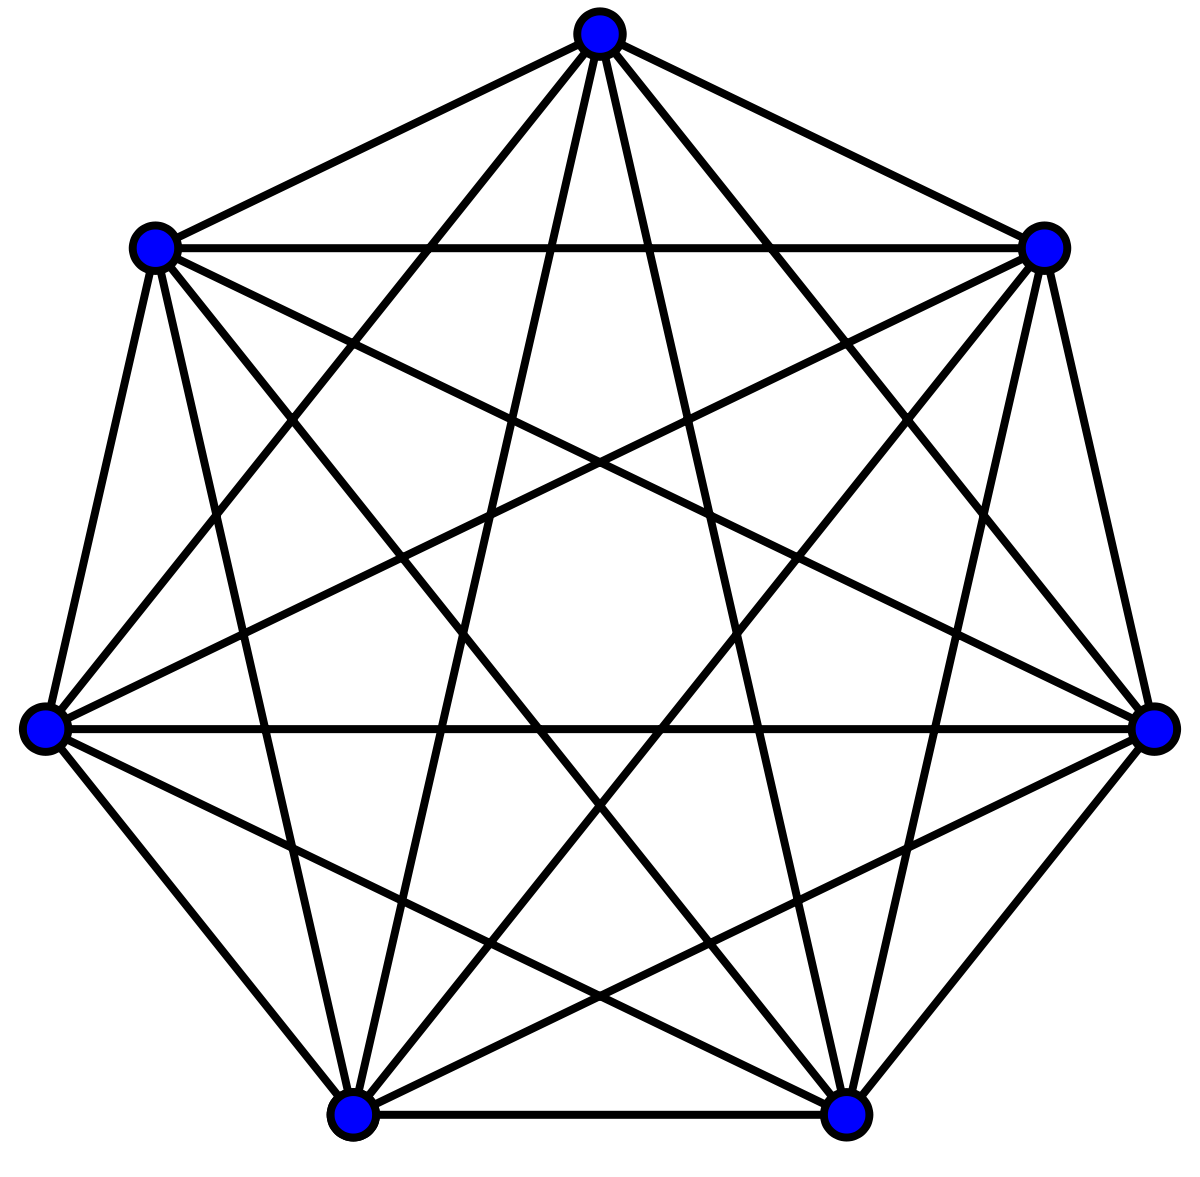
\includegraphics[width=0.3\textwidth]{K7.png}
    \caption*{Representación gráfica del grafo completo $K_7$.}
\end{figure}

\subsection{Generalizaciones}

Algunas generalizaciones\footnote{No se estudian mucho en la materia.} de los grafos son:
\begin{itemize}
    \item \textbf{Multigrafos}: En un multigrafo, $E$ pasa a ser un multiconjunto, es decir, pueden haber varias aristas entre un mismo par de vértices.
    \item \textbf{Pseudografo}: Los pseudografos pueden tiene varias aristas entre un mismo par de vértices, y también puede haber aristas que unan a un mismo par de vértices (llamadas \textit{loops}).
\end{itemize}

\subsection{Recorridos}

\begin{itemize}
    \item Un \textit{recorrido} en un grafo es una secuencia de vértices $P = v_0 v_1 \cdots v_k$ tal que todos los pares consecutivos son adyacentes, es decir, $(v_i, v_{i+1}) \in E\ \forall i = 0, ..., k - 1$. Para multi- y pseudo-grafos, se debe especificar entre qué aristas se pasa.
    \item Un \textit{camino}\footnote{Hay ambigüedad en el término: a veces se llama camino a los recorridos, en cuyo caso a los recorridos sin vértices repetidos se les dice \textit{camino simple}.} es un recorrido que no pasa por el mismo vértice $2$ veces.
    \item Una \textit{sección} de un recorrido $P$ es una subsecuencia $S = v_i v_{i+1} \cdots v_j$ de vértices consecutivos de $P$, y se denota $P_{v_i v_j}$.
    \item Un \textit{circuito} es un recorrido que empieza y termina en el mismo vértice.
    \item Un \textit{ciclo} o \textit{circuito simple} es un circuito de $3$ o más vértices que no pasa $2$ veces por el mismo vértice (salvo por el principio y fin).
\end{itemize}

\begin{figure}[H]
    \centering
    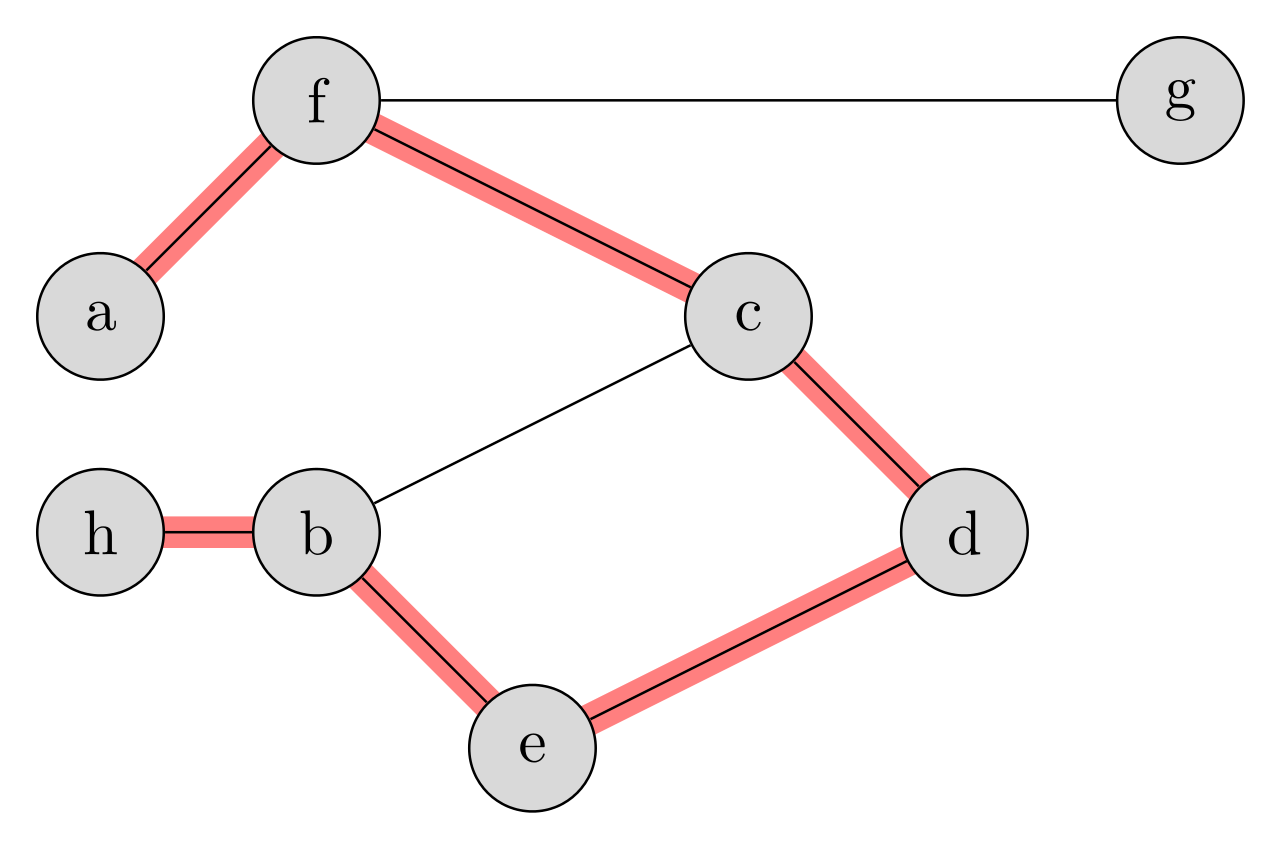
\includegraphics[width=0.3\textwidth]{ejemplo_camino.png}
    \caption*{Un ejemplo de un camino entre los vértices $a$ y $h$.}
\end{figure}

\subsection{Distancia}

Dado un recorrido $P$, su \textit{longitud}, $l(P)$, es la cantidad de aristas que tiene. Luego, la \textit{distancia} entre $v$ y $w$ se define como la longitud del camino más corto entre $v$ y $w$, y se llama $d(v, w)$. Si no hay recorrido entre $v$ y $w$, se define que $d(v, w) = \infty$, mientras que $d(v, v) = 0$ para cualquier $v$.

\begin{theorem*}
    Si un recorrido $P$ entre $v$ y $w$ cumple $l(P) = d(v, w)$, entonces es un camino.
\end{theorem*}
\begin{proof}
    Se puede demostrar por el absurdo: si $P$ no fuera un camino, tendría algún vértice $u$ por el que se pasa $2$ veces: $P = v \cdots u \cdots u \cdots w$. Si se forma un nuevo recorrido $P' = P_{vu} + P_{uw}$ (excluyendo el recorrido de $u$ a sí mismo), este tendría una longitud estrictamente menor que $P$, y por ende $l(P') < d(v, w)$ (\textbf{Absurdo}).

\end{proof}

\begin{theorem*}
    Para cualquier grafo $G = (V, E)$, la función de distancia $d: V \times V \longrightarrow \N$ es una métrica, es decir, cumple las siguientes propiedades para todo $u, v, w \in V$:
    \begin{itemize}
        \item $d(u, v) = 0 \iff u = v$
        \item $d(u, v) = d(v, u)$
        \item $d(u, w) \leq d(u, v) + d(v, w)$ (desigualdad triangular)
    \end{itemize}
\end{theorem*}
\begin{proof}
    Se demuestra por separado:
    \begin{itemize}
        \item La ida vale por definición, y la vuelta vale porque cualquier camino entre un par de vértices tiene al menos $1$ arista (y por ende $d(u, v) \geq 1$).
        \item En un grafo las aristas no tienen sentido, así que cualquier camino puede ser invertido para formar un camino válido. Por ende, la longitud del camino más corto entre $u$ y $v$ debe ser la misma que entre $v$ y $u$.
        \item Si $P_{uv}$ y $P_{vw}$ son caminos tales que $l(P_{uv}) = d(u,v)$ y $l(P_{vw}) = d(v,w)$, se pueden concatenar para formar un recorrido $P_{uv} + P_{vw}$ entre $u$ y $w$. Como la distancia es la longitud mínima entre todos los recorridos, se tiene $d(u, w) \leq l(P_{uv} + P_{vw}) = d(u, v) + d(v, w)$.
    \end{itemize}

\end{proof}

\subsection{Subgrafos}
\label{subgrafos}

Dado un grafo $G = (V_G, E_G)$,

\begin{itemize}
    \item Un \textit{subgrafo} de $G$ es un grafo $H = (V_H, E_H)$ tal que $V_H \subseteq V_G$ y $E_H \subseteq E_G \cap (V_H \times V_H)$. Los notamos como $H \subseteq G$.
    \item $H$ es un \textit{subgrafo propio} cuando $H \subseteq G$ y $H \neq G$.
    \item $H$ es un \textit{subgrafo generador} cuando $H \subseteq G$ y $V_H = V_G$.
    \item $H$ es un \textit{subgrafo inducido} cuando $(v, w) \in E_H \iff v,w \in V_H \land (v, w) \in E_H$. Estos subgrafos pueden definirse únicamente por su conjunto de vértices, y se denota como $G_{[V_H]}$.
\end{itemize}

\subsection{Conectividad}

Un grafo se denomina \textit{conexo} cuando existe un camino entre todo par de vértices. Una \textit{componente conexa} de un grafo es un subgrafo inducido conexo maximal (no se pueden agregar más vértices y mantenerlo conexo) de $G$.

Por otro lado, una arista de $G$ es \textit{puente} si $G - e$ tiene más componentes conexas que $G$.

\begin{figure}[H]
    \centering
    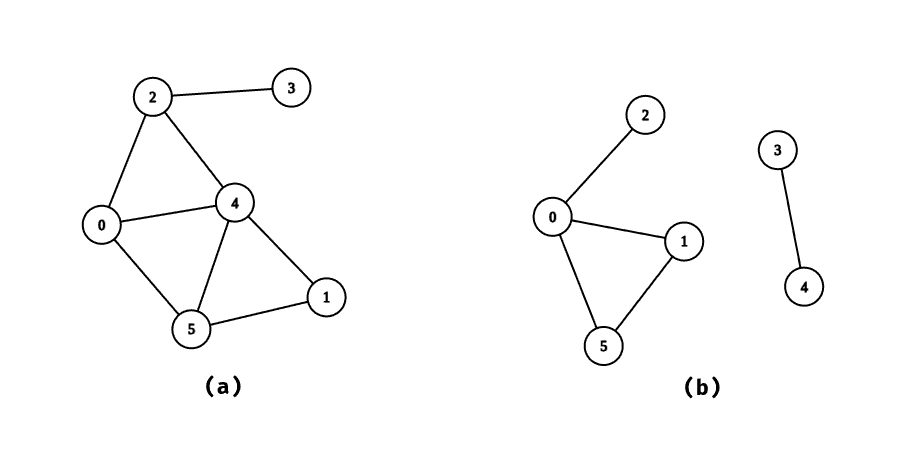
\includegraphics[width=0.5\textwidth]{ejemplo_conexo.png}
    \caption*{Un grafo conexo (a) y uno disconexo (b).}
\end{figure}

\subsection{Representación de Grafos}
\label{representacion-grafos}

Existen distintas alternativas para representar grafos en un algoritmo, que proveen ventajas y desventajas a la hora de realizar diversas operaciones.

\subsubsection{Lista de aristas}

El grafo se almacena como una lista de pares de vértices, que representan sus aristas. Esta es la forma más simple de representarlo, y es el formato que se asume que tiene la entrada de cualquier algoritmo de grafos. Debido a su falta de estructura, realizar la mayoría de las operaciones resulta costoso, con la excepción de agregar nodos o aristas.

Esta estructura tiene ciertas variaciones. Por ejemplo, se pueden ordenar los vértices dentro de cada lista, lo cual permite usar búsqueda binaria para comprobar la pertenencia de un vértice a ellas, pero aumenta la complejidad de construir la estructura y la de agregar vértices (porque hay que mantener el orden).

\subsubsection{Listas de adyacencia}

Se mantienen $n$ listas, donde cada lista $L_i$ contiene todos los vértices de $N(v_i)$. Esto permite realizar algunas operaciones más rápidamente, y la estructura se puede construir a partir de la lista de aristas en tiempo lineal.

\subsubsection{Matriz de adyacencia}

En este caso, se tiene una matriz $M \in \{0, 1\}^{n \times n}$, donde cada posición está determinada por:
$$
    M_ij =
    \begin{cases}
        1 & \si (i, j) \in E \\
        0 & \ecc
    \end{cases}
$$

La matriz es simétrica para grafos, pero no necesariamente para digrafos.

La estructura permite comprobar si dos vértices son adyacentes en tiempo constante. Sin embargo, construirla a partir de una lista de adyacencia es una operación de complejidad cuadrática, y la estructura es muy rígida (para agregar un vértice se debe armar una nueva matriz). Además, la complejidad espacial es también \BigO{|V|^2}, lo cual es problemático para guardar grafos ralos\footnote{Un grafo \textit{ralo} es uno con ``pocas'' aristas.}.

\subsubsection{Matriz de incidencia}

Esta estructura es una matriz $I \in \{0, 1\}^{m \times n}$ donde las filas representan los vértices y las columnas las aristas. Una posición $i, j$ tiene uno cuando la arista de la columna $j$ es incidente al vértice de la fila $i$.

\subsubsection{Complejidades}

% TODO: Tabla de complejidades

\subsection{Isomorfismo}

Dos grafos $G = (V, E)$ y $G' = (V', E')$ son \textit{isomorfos} cuando existe una función biyectiva $f: V \longrightarrow V'$ tal que:
$$\forall v, w \in V,\ (v, w) \in E \iff (f(v), f(w)) \in E'$$

A la función $f$ se la llama isomorfismo, y se denota $G \approxeq G'$ o (por abuso de notación) $G = G'$.

\begin{theorem*}
    Si dos grafos $G \approxeq G'$ son isomorfos.
    \begin{itemize}
        \item Tienen el mismo número de vértices.
        \item Tiene el mismo número de aristas.
        \item $\forall 0 \leq k \leq n - 1,$ tienen el mismo número de vértices de grado $k$.
        \item Tienen el mismo número de componentes conexas.
        \item $\forall 0 \leq k \leq n - 1,$ tienen el mismo número de caminos simples de longitud $k$.
    \end{itemize}
\end{theorem*}
\begin{proof}
    % TODO

\end{proof}

\subsection{Definiciones en digrafos}

\subsubsection{Vecinos}

\begin{itemize}
    \item Para un arco $e = (v, w) = v \rightarrow w$, se llama \textit{cola} de $e$ a $v$ y \textit{cabeza} de $e$ a $w$.
    \item El \textit{grado de entrada} $d_-(v)$ es la cantidad de arcos que tienen a $v$ como cabeza.
    \item El \textit{grado de salida} $d_+(v)$ es la cantidad de arcos que tienen a $v$ como cola.
    \item El \textit{grafo subyacente} de $G$ es el grafo que resulta de ignorar las direcciones de sus arcos.
\end{itemize}

\subsubsection{Recorridos}
\label{recorridos-digrafos}

\begin{itemize}
    \item Un \textit{recorrido/camino orientado} en un digrafo es una sucesión de vértices que están conectados apropiadamente por arcos (sin repetidos en el caso del camino).
    \item Un \textit{circuito/ciclo orientado} es un recorrido/camino orientado que empieza y termina en el mismo vértice.
    \item Un digrafo es \textit{fuertemente conexo} si para todo par de vértices $v, u$ existen caminos orientados de $u$ a $v$ y de $v$ a $u$.
\end{itemize}

\section{Grafos Bipartitos}

Un grafo $G = (V, E)$ es \textit{bipartito} cuando existe una \textit{bipartición} de sus vértices $(V_1, V_2)$ tal que todas las aristas de $G$ tienen un extremo en $V_1$ y el otro en $V_2$. Por otro lado, $G$ es \textit{bipartito completo} cuando todo vértice de $V_1$ es adyacente a todo vértice de $V_2$, y se denota $G = K_{|V_1|,|V_2|}$.

\begin{figure}[H]
    \centering
    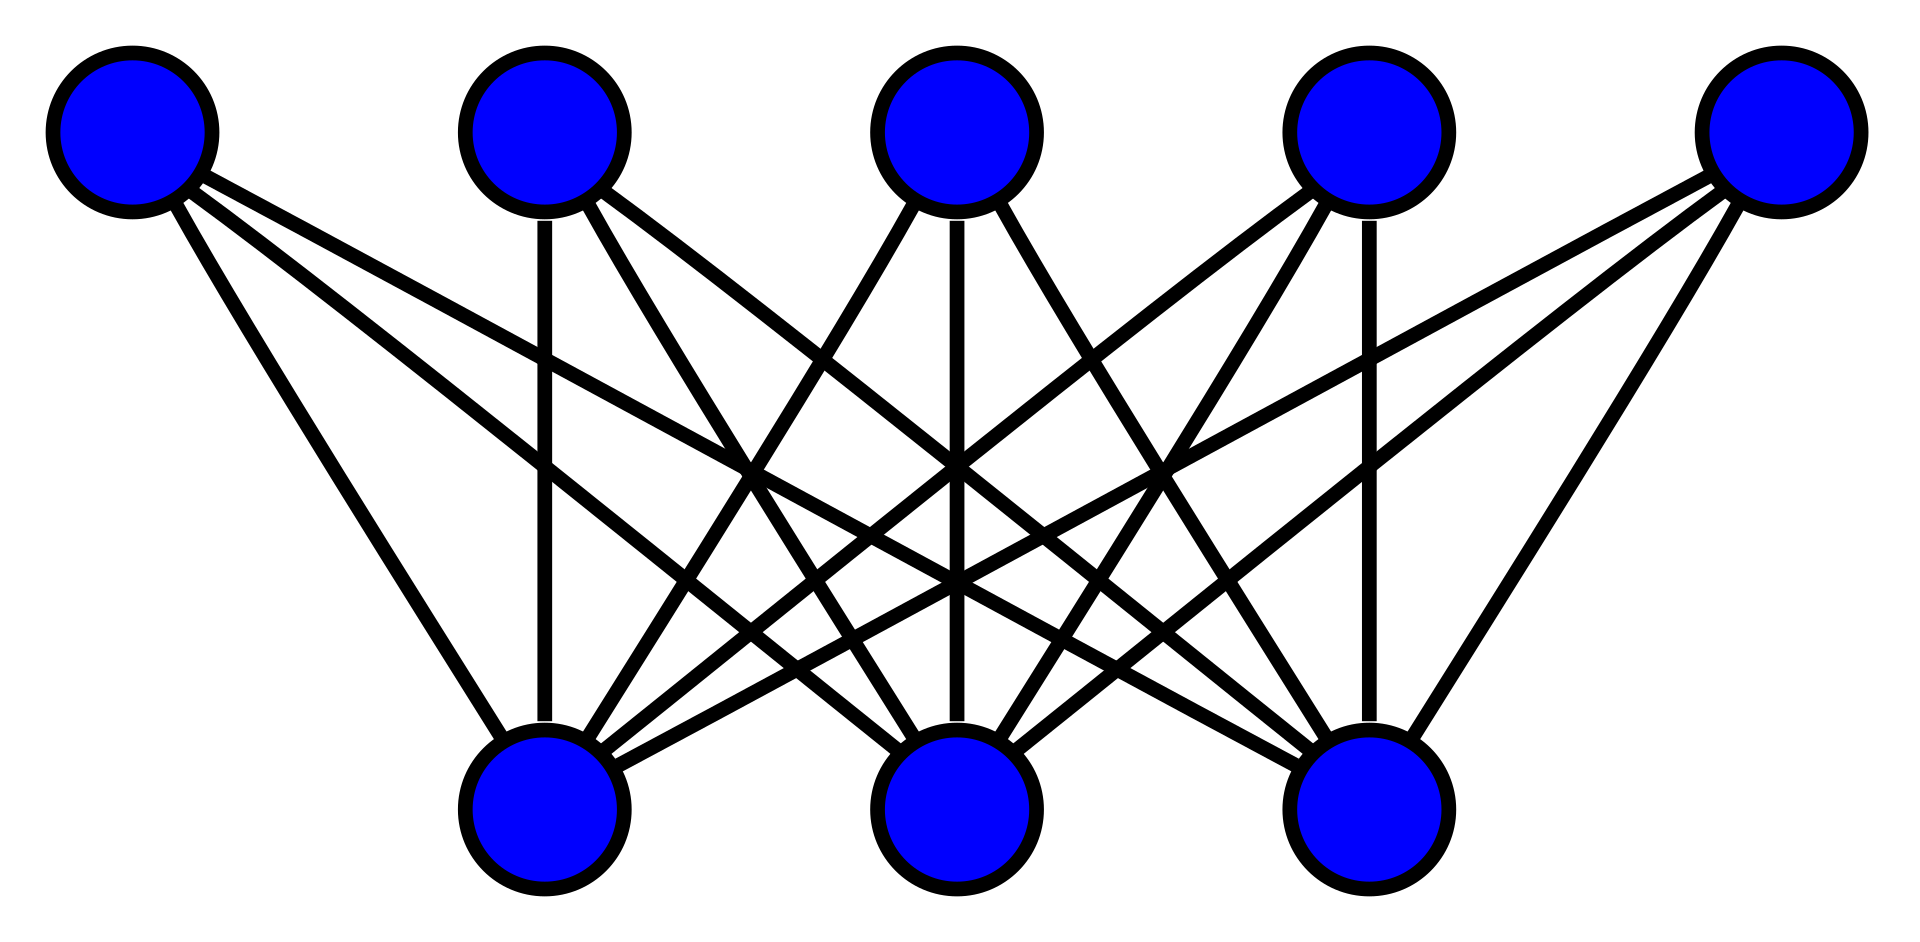
\includegraphics[width=0.3\textwidth]{grafo_K_3,5.png}
    \caption*{El grafo bipartito completo $K_{3,5}$.}
\end{figure}

\begin{theorem*}
    Un grafo $G$ es bipartito $\iff$ no tiene ciclos de longitud impar.
\end{theorem*}
\begin{proof}
    Como un grafo es bipartito si y solo si cada una de sus componentes conexas es bipartita, y un grafo no tiene ciclos impares si y solo si ninguna de sus componentes conexas tiene ciclos impares, alcanza con demostrar el teorema para grafos conexos.

    $\implies$) Sea $(V_1, V_2)$ la bipartición de $G$.

    Si $G$ tiene algún ciclo $C = v_1v_2 \cdots v_kv_1$, se puede asumir sin pérdida de generalidad que $v_1 \in V_1$. Luego, como $v_1v_2 \in E$ (y $G$ es bipartito), $v_2 \in V_2$. En general, $v_{2i+1} \in V_1$ y $v_{2i} \in V_2$. Como $v_1 \in V_1$ y $v_kv_1 \in E$, se debe cumplir $v_k \in V_2$. Por ende $k = 2i$ así que $l(C)$ es par.

    $\impliedby$) Sea $u$ cualquier vértice de $V$. Se definen los siguientes conjuntos:
    \begin{align*}
        V_1 & = \{v \in V \mid 2 \mid d(u, v)\} \cup \{u\} \\
        V_2 & = \{v \in V \mid 2 \nmid d(u, v)\}
    \end{align*}

    $(V_1,V_2)$ definen una partición de $V$. Se puede demostrar que es una bipartición de $G$ por el absurdo.

    Supongamos que no es una bipartición, entonces existen $v, w \in V_1$ (s.p.g.) tales que $vw \in E$. Si $v = u$, entonces $d(v,u) = 1$, que es absurdo porque $d(v, w)$ es par. Lo mismo vale para $w$, así que $v \neq u$ y $v \neq w$.

    Sea $P$ un camino mínimo entre $v$ y $u$ y $Q$ uno entre $v$ y $w$. Como $u, w \in V_1$ $P$ y $Q$ tienen longitud par. Luego, sea $z$ el vértice común a $P$ y $Q$ tal que $P_{zv}$ y $Q_{zw}$ son disjuntos (ignorando $z$).

    Se debe cumplir $d(u, z) = l(P_{uz}) = l(Q_{uz})$, porque del contrario $P$ y $Q$ no serían caminos mínimos. Esto implica que $l(P_{zv})$ y $l(Q_{zw})$ tienen la misma paridad, porque $l(P)$ y $l(Q)$ son ambos pares y la diferencia entre las longitudes totales y las de los subcaminos es la misma. Por ende, el ciclo $P_{zv}(v, w)Q_{wz}$ tiene longitud impar (\textbf{Absurdo}).

\end{proof}

\section{Árboles}

\subsection{Definición}

Un \textit{árbol} es un grafo conexo acíclico.

\begin{figure}[H]
    \centering
    \includegraphics*[width=0.5\textwidth]{ejemplos_arboles.png}
    \caption*{Ejemplos de grafos que son árboles.}
\end{figure}

Existen caracterizaciones alternativas:

\begin{theorem*}
    Dado un grafo $G = (V, E)$, son equivalentes:
    \begin{enumerate}
        \item G es un árbol (un grafo conexo acíclico).
        \item G es un grafo acíclico y $\forall e \notin X,$ $G + e = (V, E \cup \{e\})$ tiene exáctamente un ciclo, y ese ciclo pasa por $e$.
        \item Existe exactamente un camino simple entre todo par de vértices de $G$.
        \item $G$ es conexo, pero si se quita cualquier arista de $G$, queda un grafo disconexo (toda arista es puente).
        \item $G$ es un grafo conexo con $|E| = |V| - 1$
        \item $G$ es un grafo acíclico con $|E| = |V| - 1$.
    \end{enumerate}
\end{theorem*}

% TODO (capaz): demostrar eso

\subsubsection{Hojas}

Una \textit{hoja} en un árbol es un vértice de grado $1$. Todo árbol \textit{no trivial} (con al menos $2$ vértices) tiene al menos $2$ hojas.

% TODO: Conseguir imagen
% \begin{figure}[H]
%     \centering
%     \includegraphics*[width=0.5\textwidth]{}
% \end{figure}

\subsubsection{Bosques}

Un \textit{bosque} es un grafo sin ciclos. Sus componentes conexas forman árboles, y se cumple $m = n - c$, donde $c$ es la cantidad de componentes conexas del bosque.

% TODO: Conseguir imagen

\subsection{Árboles enraizados}

Un \textit{árbol enraizado} es un árbol con un vértice especial $r$ designado \textit{raíz}. Luego, queda definido un árbol dirigido, donde los arcos van desde vértices más cercanos a la raíz hacia los más lejanos. En tal caso, está la siguiente terminología:
\begin{itemize}
    \item Los vértices \textit{internos} son aquellos que no son ni hojas ni raíz.
    \item El \textit{nivel} de un vértice $v$ es la distancia de la raíz a ese vértice ($d(r, v)$).
    \item Para cada arco $v \rightarrow w$, $v$ es el \textit{padre} de $w$, y $w$ es el \textit{hijo} de $v$.
    \item La \textit{altura} $h$ de un árbol enraizado es la distancia desde la raíz al vértice más lejano ($\max{\{d(r, v) \mid v \in V\}}$).
    \item Un árbol se dice \textit{$m$-ario} si todos sus nodos internos tiene grado a lo sumo $m + 1$ y la raíz tiene grado a lo sumo $m$.
    \item Un árbol es \textit{balanceado} cuando la diferencia entre el nivel de cada par de hojas es a lo sumo $1$.
\end{itemize}

\begin{theorem*}
    Dado un árbol enraizado $m$-ario con altura $h$ y $l$ hojas, $l \leq m^h$ ($\iff h \geq \lceil\log_m{l}\rceil$).
\end{theorem*}

% TODO: Demostración

\subsection{Representación de árboles}

Además de las representaciones de grafos \hyperref[representacion-grafos]{anteriormente mencionadas}, los árboles enraizados tienen una alternativa particular: debido a que todos los nodos tienen un único padre, un árbol puede ser definido por la correspondencia entre cada nodo y su antecesor. Esto se puede lograr usando solamente un arreglo ``\code{prev}'', en el que cada posición $i$ contiene al padre del nodo $v_i$. La única excepción es la raíz $r$ que, al no tener antecesor, se puede marcar utilizando un valor especial $\perp$, o como su propio padre ($d[r] = r$)\footnote{Esto se puede extender para guardar bosques: basta con tener varias raíces.}.

\subsection{Árbol generador}
\label{arbol-generador}

Un \textit{árbol generador} (AG) de un grafo $G$ es un \hyperref[subgrafos]{subgrafo generador} que además es un árbol. En la práctica, los árboles generadores son utilizados cuando se busca conectar (con la cantidad mínima posible de conexiones) a $n$ puntos (ciudades, centrales eléctricas, servidores).
\begin{theorem*}
    Dado un grafo conexo $G = (V, E)$.

    \begin{itemize}
        \item $G$ tiene (al menos) un árbol generador
        \item $G$ tiene un único árbol generador $\iff$ $G$ es un árbol.
        \item Sea $T = (V, E_T)$ un AG de $G$ y $e \in E - E_T$. Luego, para toda arista $f \neq e$ contenida en el único ciclo de $T + e$, $T + e - f = (V, E_T \cup \{e\} - \{f\})$ es un AG de $G$.
    \end{itemize}
\end{theorem*}

\section{Recorridos}
\label{recorridos}

Es común querer pasar por todos los vérices de un grafo una única vez. Existen distintos métodos de hacerlo de forma sistemática y ordenada, y en este caso nos vamos a enfocar en los $2$ más comunes: \textit{BFS} y \textit{DFS}. En ambos casos, se mantiene una \textit{frontera} con los vértices que se están por explorar, y cada vez que se pasa por uno de ellos sus vecinos son agregados a la misma. Además, se mantiene un conjunto de los vértices explorados (generalmente implementado con un \textit{bitset}) para evitar su repetición. El esquema general es el siguiente:

\begin{codebox}
    \Procname{$\proc{Recorrer}(G, s)$}
    \li Inicializar la frontera $F = \{s\}$.
    \li \While la frontera no esté vacía \Do
    \li Extraer un $v$ de la frontera.
    \li $\proc{Procesar}(v)$
    \li \For \Each $u \in N(v)$ \Do
    \li \If $u$ no fue visitado \Then
    \li Marcar a $u$ como visitado.
    \li Agregar $u$ a la frontera.
    \End
    \End
    \End
\end{codebox}

\subsection{BFS}

El \textit{Breadth-First Search} (BFS) es un algoritmo que, dado un grafo $G$ y un vértice inicial $s$, recorre todos los vértices nivel por nivel, es decir, los vértices más cercanos al inicial son visitados primero. Formalmente, si $\langle v_1, ..., v_n \rangle$ es la secuencia de vértices en el orden en que son recorridos, entonces se cumple:
$$d(s, v_i) \leq d(s, v_j)\ \forall\,1 \leq i \leq j \leq n$$

Para lograr esto, BFS utiliza como frontera una cola, donde los elementos son procesados en orden de llegada (FIFO). El algoritmo se puede implementar iterativamente de la siguiente manera:

\begin{codebox}
    \Procname{$\proc{BFS}(G = (V, E), s)$}
        \li $\id{visitados} \gets \emptyset$
        \li Inicializar árbol $T$ con raíz en $s$.
        \li Inicializar arreglo de distancias $d$.
        \li Inicializar cola $Q$.
        \li $d[s] \gets 0$
        \li $\proc{Encolar(Q, s)}$
        \li \While $\neg\proc{Vacío?}(Q)$ \Do
        \li $v \gets \proc{Desencolar}(Q)$
        \li $\proc{Procesar}(v)$
        \li \For \Each $u \in N(v)$ \Do
        \li \If $u \notin \id{visitados}$ \Then
        \li $\id{visitados} \gets \id{visitados} \cup \{u\}$
        \li $d[u] \gets d[v] + 1$
        \li Agregar $u$ a $T$ como hijo de $v$.
        \li $\proc{Encolar}(Q, u)$
        \End
        \End
        \End
        \li \Return $(T, d)$
\end{codebox}

El algoritmo devuelve $2$ valores: un árbol generador $T$, que se denomina \textit{árbol BFS} y contiene las aristas transitadas por el recorrido, junto con la función $d: V \longrightarrow \N_0$, que indica las distancias de $s$ a cada vértice del grafo.

Si el grafo se representa utilizando listas de adyacencia, el vecindario $N(v)$ se puede recorrer fácilmente. El algoritmo pasa una sola vez por cada vértice y, asumiendo que tanto $\id{visitados}$, $T$ y $d$ se representan a través arreglos, realiza una operación de tiempo constante en cada uno de sus vecinos. Por ende, la complejidad de este algoritmo es:
$$\BigO{|V| + \sum_{v \in V} d(v)} = \BigO{|V| + 2|E|} = \BigO{|V| + |E|}$$

\subsubsection{Árboles geodésicos}

Un árbol generador $T$ de un grafo $G$ se llama $v$-geodésico cuando $d_G(v, w) = d_T(v, w)\ \forall w \in V$.
\begin{theorem*}
    Si se corre el algoritmo BFS en un grafo $G$ empezando en un vértice $s$, el árbol generador resultante $T$ es $s$-geodésico, y las distancias que devuelve son las mínimas entre $s$ y cada vértice del árbol.
\end{theorem*}
\begin{proof}
    % TODO
\end{proof}

\subsection{DFS}

La estrategia que sigue el \textit{Depth-First Search} (DFS) es buscar ``en profundidad'' siempre que sea posible. Esto significa que al llegar a $v$, se recorren todos los vértices no visitados alcanzables desde este. Este procedimiento se realiza hasta que todos los nodos hayan sido explorados.

El algoritmo de DFS se puede implementar recursivamente de la siguiente manera (\id{visitados}, $T$, \id{principio}, \id{fin} y \id{contador} son variables globales):

\begin{codebox}
    \Procname{$\proc{DFS}(G, s)$}
    \li $\id{visitados} \gets \emptyset$
    \li $\id{contador} \gets 0$
    \li Inicializar arreglos \id{principio} y \id{fin}.
    \li Inicializar $T$ como árbol vacío.
    \li $\proc{Visitar-DFS}(G, s)$
\end{codebox}
\label{dfs-visit}
\begin{codebox}
    \Procname{$\proc{Visitar-DFS}(G, v)$}
    \li $\id{contador} \gets \id{contador} + 1$
    \li $\id{principio}[v] \gets contador$
    \li $\id{visitados} \gets \id{visitados} \cup v$
    \li \For \Each $u \in N(v)$ \Do
    \li \If $u \notin \id{visitados}$
    \li Agregar $u$ como hijos de $v$ en el árbol $T$.
    \li $\proc{Visitar-DFS}(G, u)$
    \End
    \End
    \li $\id{contador} \gets \id{contador} + 1$
    \li $\id{fin}[v] \gets \id{contador}$
\end{codebox}

El tiempo de ejecución del algoritmo, al igual que BFS, es lineal\footnote{La linealidad de estas complejidades se refiere a que, como los grafos se pasan como listas de adyacencia, el tamaño de la entrada es $|E|$. Si se considerara la cantidad de vértices, una complejidad de \BigO{|E|} sería cuadrática, ya que $|E| \in \BigO{|V|^2}$.}: hay una llamada por cada nodo, y cada llamada tiene un tiempo de ejecución proporcional al grado del nodo, así que la complejidad es $\BigO{|V| + |E|}$.

Al terminar, DFS no solo devuelve el árbol generado $T$, sino que también un par de arreglos \id{principio} y \id{fin}. El primero guarda el orden en el que se empieza a explorar el subárbol de cada nodo (también llamado \textit{pre-order}), mientras que el segundo guarda el orden en el que se termina dicha exploración (también llamado \textit{post-order}). Estos valores son muy útiles para analizar la estructura del árbol.

\begin{theorem*}
    Dado grafo $G$ y un árbol DFS $T_G$ y un par de vértices $v$, $u$, se cumple alguna de las siguientes:
    \begin{enumerate}
        \item $[\id{principio}[v], \id{fin}[v]] \cap [\id{principio}[u], \id{fin}[u]] = \emptyset$, y en tal caso $v$ y $u$ están en ramas distintas (ninguno es descendiente del otro).
        \item $[\id{principio}[v], \id{fin}[v]] \subseteq [\id{principio}[u], \id{fin}[u]]$, y entonces el vértice $v$ es descendiente de $u$.
        \item $[\id{principio}[v], \id{fin}[v]] \supseteq [\id{principio}[u], \id{fin}[u]]$, y entonces el vértice $u$ es descendiente de $v$.
    \end{enumerate}
\end{theorem*}

\subsubsection{Tipos de aristas}
\label{dfs-edges}

Dado un grafo $G$ y un árbol DFS $T$, las aristas de $G$ se pueden dividir en las siguientes categorías:
\begin{itemize}
    \item \textit{Tree edges}: son aquellas que están en $E_T$.
    \item \textit{Back edges}: son aquellas que no están en $E_T$, y que conectan a un nodo con un antecesor en $T$.
    \item \textit{Forward edges}: son aquellas que no están en $E_T$, y que conectan a un nodo con un descendiente en $T$.
    \item \textit{Cross edges}: son aquellas que no están en $E_T$, y que conectan a nodos de distintas ramas del árbol.
\end{itemize}

La categoría de cualquier arista puede ser identificada en tiempo constante utilizando los resultados del DFS: la pertenencia a $E_T$ se puede chequear revisando los padres de los vértices incidentes a la arista en el árbol, mientras que las otras condiciones se pueden verificar a través de los arreglos \id{principio} y \id{fin}.
\begin{theorem*}
    Dado un grafo \underline{no dirigido} $G$, todas las aristas de cualquier árbol DFS son Tree Edges o back edges.
\end{theorem*}

\subsubsection{Detección de ciclos}

\begin{theorem*}
    Un grafo $G$ es acíclico $\iff$ ningún árbol DFS de $G$ tiene back edges.
\end{theorem*}
\begin{proof}
    \leavevmode

    $\implies$) Se demuestra por el contrarrecíproco: si $T$ es un árbol DFS con una backedge $e = u \rightarrow v$, se puede tomar el ciclo $C = P + e$, donde $P$ es el camino que une a $v$ y $u$ en $T$ (debe existir, ya que $v$ es antecesor de $u$ por ser $e$ back edge).

    $\impliedby$) También se demuestra el contrarrecíproco: supongamos que $C$ es un ciclo de $G$. Dado un recorrido DFS cualquiera, sea $v$ el primer vértice de $C$ que se encuentra y $u$ el vértice ``anterior''\footnote{En grafos no dirigidos hay dos: se puede tomar sin pérdida de generalidad.} en el ciclo. Luego, como $u$ es alcanzable desde $v$, será uno de sus descendientes, así que la arista $u \rightarrow v$ es una back edge.

\end{proof}

El algoritmo DFS puede ser utilizado para encontrar ciclos de un grafo, ya que todas las back edges forman parte de al menos un ciclo. Existen varias opciones:
\begin{itemize}
    \item En el caso de los grafos no dirigidos, basta con adaptar DFS para devolver el ciclo cuando un vértice $u$ adyacente al actual $v$ ya fue visitado. En ese caso, el ciclo es $C = uT_{uv}vu$, donde $T_{uv}$ es el camino entre $u$ y $v$ en el árbol. Esto funciona porque cuando se visita un vértice por segunda en un grafo no dirigido vez siempre se hace a través de una Back Edge.
    \item Otra opción que también sirve para grafos dirigidos es pasar por todas las aristas que no están en el árbol hasta identificar una Back Edge (usando las condiciones \hyperref[dfs-edges]{establecidas anteriormente})
\end{itemize}

\subsubsection{Versión iterativa}

La versión iterativa de DFS sigue el esquema general \hyperref[recorridos]{establecido previamente}. En este caso, la frontera se implementa utilizando un stack (FILO), lo cual garantiza que un vértice se deja de explorar solo cuando todos los vértices alcanzables desde ese fueron visitados.

\subsubsection{Bosques}

Si el grafo recorrido $G$ no es conexo, se puede formar un bosque donde cada componente conexa es un árbol DFS. Esto se logra corriendo DFS iterativamente, cada vez empezando en uno de los vértices que aún no fue recorrido por las iteraciones anteriores. El algoritmo es el siguiente, donde \proc{Visitar-DFS} es el procedimiento definido anteriormente:

\begin{codebox}
    \Procname{$\proc{DFS}(G)$}
    \li $\id{visitados} \gets \emptyset$
    \li $\id{contador} \gets 0$
    \li Inicializar arreglos \id{principio} y \id{fin}.
    \li Inicializar $T$ como árbol vacío.
    \li \For \Each $v \in V$ \Do
    \li \If $v \notin \id{visitados}$ \Then
    \li $\proc{Visitar-DFS}(G, s)$
    \End
    \End
\end{codebox}

\section{Orden Topológico}
\label{orden-topologico}

\subsection{Definición}

\begin{problema}
    Dado un digrafo acíclico (un ``DAG'') $D = (V, E)$, encontrar un ordenamiento $\langle v_1, v_2, ..., v_n \rangle$ de sus vértices de forma tal que, para todo $v \in V$ los vértices alcanzables desde $v$ aparezcan después en el orden. Formalmente,
    $$d(v_i, v_j) < \infty \implies\ \forall\ 1 \leq i \leq j \leq n$$
\end{problema}

Esto se denomina un \textit{orden/ordenamiento topológico}, y tiene múltiples aplicaciones prácticas, que surgen cada vez que se debe ordenar un conjunto de cosas con precedencias entre sí. Notar que solo es posible para digrafos acíclicos: en un ciclo, todos los vértices son alcanzables desde los demás, así que ninguno podría ir antes de los demás.

\subsection{Algoritmo}

Habiendo implementado y analizado DFS, el algoritmo para encontrar un ordenamiento topológico es simple, gracias al siguiente teorema:

\begin{theorem*}
    Para un DAG $D$, el ordenamiento inverso al post-order de cualquier DFS es un orden topológico.
\end{theorem*}
\begin{proof}
    Como el valor de \id{fin}[$v$] se asigna después de haber explorado por todos los vértices $u$ alcanzables desde $v$, se cumple que $\id{fin}[u] < \id{fin}[v]$. Por ende, si se ordenan los vértices por valor \id{fin} decreciente, los vértices que se pueden alcanzar desde otros aparecerán después.
\end{proof}

Para implementar este algoritmo, no es necesario ordenar directamente los vértices a través de \id{fin} (lo tendría complejidad \BigO{|V|\log{|V|}}), sino que basta con modificar DFS: después de terminar de explorar el subárbol de cada vértice, se lo agrega al principio de una secuencia. Esto produce un ordenamiento topológico de $D$.

\section{Algoritmo de Kosaraju}

El algoritmo de Kosaraju es un algoritmo lineal que encuentra las \hyperref[recorridos-digrafos]{componentes fuertemente conexas} de un digrafo $G$. Se basa en hacer $2$ recorridos DFS: el primero se utiliza para obtener un post-order de los vértices del grafo, mientras que el segundo lo recorre de manera inversa para armar los componentes. Este segundo DFS se hace sobre $G^T$, el digrafo cuyas aristas tienen el sentido opuesto al de las de $G$. El algoritmo es el siguiente:

\begin{codebox}
    \Procname{$\proc{Kosaraju}(G)$}
    \li Llamar a $\proc{DFS}(G)$ para obtener un post-order inverso.
    \li Computar $G^T$
    \li Llamar a $\proc{DFS}(G^T)$, pero en el loop principal explorar los vértices en el post-order inverso.
    \zi Cada vez que se visita un vértice nuevo, agregarlo a la CFC de la raíz actual.
\end{codebox}

El loop principal de DFS se refiere al de la versión que arma bosques iterando por cada vértice sin explorar.

Para ver por qué este algoritmo funciona, primero se debe observar el siguiente lema:
\begin{lemma*}
    Dadas CFCs\footnote{Componentes Fuertemente Conexas} $C$ y $C'$ distintas en $G = (V, E)$, ningún vértice de $C$ es alcanzable desde $C'$, o viceversa.
\end{lemma*}
\begin{proof}
    Esto se puede demostar por el absurdo: si existen caminos $u \leadsto v$ y $u' \leadsto v'$ tales que $u, v \in C$ y $u', v' \in C'$, entonces cualquier vértice de $C$ puede llegar a cualquiera de $C'$ a pasando por $u \leadsto v$, y cualquiera de $C'$ puede a su vez llegar a uno de $C$ a través de $u' \leadsto v'$. Esto implica que todos están en la misma CFC (\textbf{Absurdo}).

\end{proof}

Esto permite visualizar las componentes conexas de un digrafo como un DAG: $G^{CFC}$ se puede definir como el grafo donde cada vértice es una versión compactada de un CFC de $G$. No puede haber ciclos porque violarían el lema anterior.

Luego, el post-order se puede emplear gracias a que:
\begin{lemma*}
    Si $C$ y $C'$ son CFCs distintas de $G$ y existe un arco $u \rightarrow v$ tal que $u \in C$ y $v \in C'$, entonces $\id{fin}[C] > \id{fin}[C']$\footnote{El \id{fin} de una CFC se define como $\max{\{\id{fin}[v] \mid v \in C\}}$.}.
\end{lemma*}
\begin{proof}
    Se puede separar en dos casos dependiendo de qué CFC se visita antes:
    \begin{itemize}
        \item Si algún vértice $w$ de $C$ se explora primero, entonces esta exploración va a alcanzar el vértice $u$ (porque están en la misma CFC), y por ende visitar todos los vértices de $C'$ antes de $\id{fin}[w]$, y por ende $\id{fin}[C] > \id{fin}[C']$.
        \item Si $C'$ se visita primero, la exploración va a concluir sin pasar por ningún vértice de $C$ ya que, gracias al lema anterior, no existen caminos entre vértices de $C'$ y los de $C$. Esto implica que $\id{fin}[C] > \id{fin}[C']$.
    \end{itemize}
\end{proof}

Esto tiene como corolario que, en el grafo $G^T$, un par de CFCs $C$ y $C'$ con un arco $u \rightarrow v$ tal que $u \in C$ y $v \in C'$ cumplen $\id{fin}[C] < \id{fin}[C']$. Eso se debe a que $G^T$ tiene los mismos CFCs que $G$, y $u \rightarrow v \in E^T \implies v \rightarrow u \in E$.

Finalmente, se puede demostrar la correctitud del algoritmo:
\begin{theorem*}
    El algoritmo de Kosaraju devuelve las componentes conexas de un digrafo $G$.
\end{theorem*}
\begin{proof}
    Como el segundo DFS empieza por un vértice $v$ de la CFC con $\id{fin}[C]$ máximo, ninguno de sus vértices contiene una arista hacia otra CFC $C'$ (porque en ese caso $\id{fin}[C] < \id{fin}[C']$). Además, como todos los vértices de $C$ son alcanzables desde $v$, la CFC se construye correctamente (se visitan todos sus vértices, y ningún otro). Luego, para las demás componentes, sucederá algo similar: las únicas aristas que las conectan con otras CFCs serán a aquellas con un mayor valor de \id{fin}, y por ende ya habrán sido exploradas. Esto implica que el algoritmo arma cada componente de forma correcta.

\end{proof}


\chapter{Árbol Generador Mínimo}

\section{Definición}

\subsubsection{Grafos pesados}

Un \textit{grafo pesado} es un grafo $G = (V, E)$ junto con una función $w: E \longrightarrow \N$, donde $w(e)$ es el peso de la arista $e$. El peso suele usarse para modelar diversas magnitudes, como el costo de una arista, o tiempo que se tarda en pasar por ella.

% TODO: Imagen

\subsubsection{AGM}

Un \textit{árbol generador mínimo} (AGM) es un \hyperref[arbol-generador]{árbol generador} cuyo peso total es menor al de todos los demás AGs, donde peso total se define como la suma de los pesos de sus aristas. Formalmente, el problema es el siguiente:

\begin{problema}
    Dado un grafo $G = (V, E)$ y una función de peso $w: E \longrightarrow \N$, encontrar un AG $T = (V, E_T)$ que cumpla:
    $$w(T) = \sum_{e \in E_T} w(e) \leq \sum_{e \in E_{T'}} w(e) = w(T')$$

    Para cualquier árbol generador $T' = (V, E_{T'})$ en $G$.
\end{problema}

También se puede definir el árbol generador máximo, que maximiza el peso total de $T$, pero este problema se puede \hyperref[reducciones]{reducir} al anterior: si se toman los pesos $w'(e) = -w(e)$, el peso  de cualquier AG $T$ será $w'(T) = \sum_{e \in E_T} w'(e) = \sum_{e \in E_T} -w(e) = -w(T)$, y por ende:
\begin{align*}
    w'(AGM) \leq w'(T) & \iff -w'(AGM) \geq -w'(T) \\
                       & \iff w(AGM) \geq w(T)
\end{align*}

\subsubsection{Propiedades}

El AGM de un grafo \underline{no necesariamente es único}: pueden varios grafos con el mismo peso, que es menor al de todos los demás.

\begin{figure}[H]
    \centering
    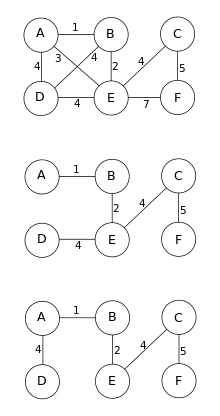
\includegraphics[width=0.3\textwidth]{ejemplo_agm.png}
    \caption*{Un grafo y 2 de sus AGMs, ambos con peso total $16$.}
\end{figure}

\subsubsection{Algoritmos}

En las siguientes secciones analizaremos $2$ algoritmos para encontrar un AGM: el algoritmo de Prim y el de Kruskal. Ambos son golosos: siguen estrategias que toman en cada paso la mejor decisión a corto plazo, y en este caso devuelven soluciones óptimas. Logran esto armando progresivamente un bosque (en el caso de Prim un árbol) en un ciclo que mantiene el invariante de que sus aristas forman un subconjunto de las de algún AGM.

\begin{codebox}
    \Procname{$\proc{Arbol-Generador-Minimo}(G, w)$}
    \li Inicializar grafo $T = (V, \emptyset)$
    \li \While $T$ no es un AG (es disconexo): \Do
    \li Encontrar una arista segura $e$.
    \li Agregar $e$ a $E_T$.
    \End
    \li \Return $T$
\end{codebox}

\label{arista-segura}
En este contexto una arista es \textit{segura} cuando se puede agregar al bosque $T$ y mantener el invariante (es un subconjunto de algún AGM). Encontrar una es donde radica la dificultad del problema, y es en donde difieren los algoritmos.

\section{Algoritmo de Prim}

\subsection{Introducción}

El \textit{algoritmo de Prim} mantiene un árbol $T = (V_T, E_T)$, y en cada iteración agrega un nuevo vértice de $V - V_T$ al mismo (junto con una arista a $E_T$), hasta que $T$ pasa por todos los vértices de $G$ (y se vuelve un AG). La arista seleccionada en cada paso es la de mínimo peso entre todas las $(u, v) \in V_T \times (V - V_T)$ (las que conectan vértices dentro del árbol con los de afuera).

Se puede implementar de la siguiente manera:

\begin{codebox}
    \Procname{$\proc{Prim}(G, w)$}
    \li $V_T \gets \{s\}$ (cualquier vértice)
    \li $E_T \gets \emptyset$
    \li \For $i \gets 1$ \To $n - 1$ \Do
    \li $e \gets \arg\min{\{w(e) \mid e = uv \in E,\ u \in V_T,\ v \in V - V_T\}}$
    \li $E_T \gets E_T \cup e$
    \li $V_T \gets V_T \cup v$
    \End
    \li \Return $T \gets (V_T, E_T)$
\end{codebox}

El algoritmo asume que el grafo es conexo. Si esto no se cumple, se puede modificar el algoritmo levemente\footnote{El único problema que tiene esa implementación es que asume que el conjunto del que se toma el $\arg\min$ no está vacío. Si esto se chequea en cada iteración, se puede terminar la ejecución cuando no quedan vértices por agregar.} para que devuelva el AGM de la componente conexa que contiene al vértice inicial.

\subsection{Correctitud}

\begin{theorem*}
    El árbol que devuelve el algoritmo de Prim es un AGM.
\end{theorem*}
\begin{proof}
    Se demuestra por inducción. La hipótesis inductiva será la siguiente: $\forall\,0 \leq k \leq n - 1, T_k = (V_k, E_k)$, el grafo mantenido por Prim en la $k$-ésima iteración del ciclo, es un árbol y es subgrafo de algún AGM de $G$.

    \textbf{Caso Base}: En el paso $k = 0$, todavía no se entró al ciclo, así que $T_0 = (\{s\}, \emptyset)$, que es un árbol (no tiene ciclos) y es subgrafo de cualquier AG (y por lo tanto de cualquier AGM).

    \textbf{Paso Inductivo}: Sea $e = vw$ agregada en la iteración. Luego, $T_k = (V_k, E_k) = (V_{k - 1} \cup \{w\}, E_{k - 1} \cup \{e\})$. Por hipótesis inductiva, se sabe que $T_{k - 1}$ es subgrafo de algún árbol generador $T$. Existen dos posibilidades:
    \begin{itemize}
        \item $e \in E_T$, en cuyo caso $T_k$ es también subgrafo de $T$.
        \item $e \notin E_T$. Aún así, sabemos que $V_{k - 1}$ forma una componente conexa en $T$, porque $T_{k - 1}$ es un subgrafo suyo y es conexo (es un árbol). Entonces, debe haber alguna arista $e' = v'w' \in E_T$ que conecta $V_{k - 1}$ y $V - V_{k - 1}$. Si se saca esa arista de $T$, las componentes se vuelven disconexas, pero se pueden volver a conectar usando la arista $e$.

              Por ende, $T' = T + e - e' = (V, (E_T \cup \{e\}) - \{e'\})$ es un árbol (y es generador, ya que contiene a todos los vértices). Además, como $e'$ era una de las aristas que se podían elegir al principio de la iteración (conecta a $V_{k - 1}$ con $V - V_{k - 1}$), se debe cumplir que $w(e) \leq w(e')$, así que:
              $$w(T') = w(T) + \underbrace{w(e) - w(e')}_{\leq 0} \leq w(T)$$

              Por lo tanto, el peso total de $T'$ es menor o igual al de un AGM, así que este también es AGM. Como $T_k$ es subgrafo de $T'$ ($E_k = E_{k - 1} \cup \{e\} \subseteq E_T \cup \{e\}, e' \notin E_k$), se cumple la propiedad.
    \end{itemize}

    Dado que la propiedad vale al terminar cualquier iteración, también se cumple en $k = n - 1$, donde $T_{k - 1}$ tiene $n$ vértices, y por lo tanto es un árbol generador (y mínimo).

\end{proof}

\subsection{Complejidad}
\label{complejidad-prim}

Para implementar el algoritmo de Prim, es necesario determinar un método para encontrar la arista de menor peso entre $V_T$ y $V - V_T$. Esto se puede lograr utilizando una cola de prioridad, pero la forma en la que esta se represente puede variar:
\begin{itemize}
    \item \underline{Un arreglo de $|V|$ posiciones}: En este caso, el peso de la arista que conecta a cada vértice con el árbol se guarda en una posición del arreglo (los vértices que ya se agregaron se marcan con un valor especial). Para determinar el siguiente vértice a agregar, se toma el mínimo del arreglo, y una vez que se agrega se actualizan las posiciones correspondientes (en caso de que uno de sus vecinos se pueda alcanzar con peso menor al anterior). Ambas operaciones son \BigO{|V|}, y como se realizan $|V| - 1$ operaciones, la complejidad total \BigO{|V|^2}.
    \item \underline{Un heap}: En este caso, se mantiene un mín-heap de los nodos que no fueron explorados, donde la clave es el peso mínimo entre las aristas que lo conectan al árbol. En cada paso se desencola un vértice, y se actualizan las claves de sus vecinos\footnote{Para lograr esto en tiempo logarítmico, es preferible usar un árbol balanceado (como los AVLs) antes que un heap.}. Esto implica que se realizan $1 + d(v)$ operaciones logarítmicas en cada iteración, lo cual resulta en una complejidad total de \BigO{(|V| + |E|)\log{|V|}}. Como se asume que $G$ es conexo, $|E| \geq |V| - 1$, y por ende $\BigO{(|V| + |E|)\log{|V|}} \subseteq \BigO{|E|\log{|V|}}$.
\end{itemize}

En el caso de los grafos \textit{densos}, que se podrían definir como aquellos en los que $|E| \in \BigOmega{|V|^2}$, la segunda alternativa tendría complejidad \BigO{|V|^2\log{|V|}}, mientras que la primera solo \BigO{|V|^2}. Por otro lado, si el grafo es \textit{ralo}, que sería cuando $|E| \in \BigO{|V|}$, la segunda sería tan solo \BigO{|V|\log{|V|}}, mejor que \BigO{|V^2|}.

Hay una tercera opción para representar la cola de prioridad: a través de Fibonacci heaps. Estos permiten que el algoritmo corra en \BigO{|E| + |V|\log{|V|}} (asintóticamente mejor que las dos anteriores), pero es más complejo de implementar que las otras opciones.

\section{Algoritmo de Kruskal}

\subsection{Disjoint-Set/Union-Find}

Antes de ver el algoritmo en sí, es necesario una de las estructuras que usa: el \textit{Disjoint-Set} o \textit{Union-Find}. Esta mantiene una partición $P_1, ..., P_n$ de un conjunto $C$, asignándole a todos los elementos de cada $P_i$ un mismo representante $r_i$. Permite realizar las siguientes operaciones de forma eficiente:
\begin{itemize}
    \item \proc{Make-Set}($x$): crea un nuevo conjunto $\{x\}$ dentro de la partición. Como precondición, $x$ no puede estar en ninguno de los conjuntos anteriores.
    \item \proc{Union}($x$, $y$): Reemplaza los conjuntos que contenían a $x$ e $y$, $S_x, S_y$ por su unión $S_x \cup S_y$.
    \item \proc{Find}($x$): Devuelve el representante $r_x$ de $x$ dentro de la partición. Esto puede ser utilizado para comprobar si dos elementos pertenecen al mismo conjunto.
\end{itemize}

\subsubsection{Implementación}

Internamente, la estructura se implementa como un bosque, donde cada árbol se corresponde con el conjunto de la partición que contiene a sus vértices, y la raíz es el representante. Implementar la operación \proc{Union} es simple: solo es necesario agregar a la raíz de uno de los conjuntos como hijo de la raíz del otro. \proc{Find} también resulta trivial: solo es necesario recorrer los antecesores de cada nodo hasta llegar a la raíz.

Esto alcanza para implementar a la estructura, pero la complejidad no es ideal: los árboles podrían ser degenerados (una línea donde cada nodo tiene $1$ solo hijo), lo cual haría que \proc{Find} sea \BigO{n}. Para evitar que suceda esto, se emplean 2 heurísticas:
\begin{itemize}
    \item \textbf{Union by rank}\footnote{Es equivalente usar la alternativa \textbf{union by size}, que usa la cantidad de nodos en el árbol en lugar de la altura.}: Esto implica mantener la altura de cada árbol guardado, lo cual en este caso no es costoso: la única forma en la que puede cambiar es cuando se agrega otro árbol $T$ a la raíz como hijo, y en tal caso la altura pasa a ser el mínimo entre la anterior y $h(T) + 1$. Esto se utiliza a la hora de decidir qué raíz utilizar para el nuevo árbol de \proc{Union}: se elige la que resulte en menor altura (queda como raíz el representante de mayor rango).
    \item \textbf{Path compression}: Esta optimización se basa en el hecho de que la estructura interna del árbol no es rígida: solo se debe cumplir que la raíz sea el representante de todos los nodos. Por ende, cada vez que se realiza un \proc{Find}, todos los vértices transitados se pueden colocar como hijos directos del árbol.
\end{itemize}

Los algoritmos se pueden implementar de la siguiente manera, donde \id{prev} es el arreglo que guarda los antecesores de cada nodo (representa al bosque) y \id{rank}[$v$] guarda la altura del árbol con raíz en $v$:
\begin{codebox}
    \Procname{$\proc{Make-Set}(x)$}
    \li $\id{prev}[x] \gets x$
    \li $\id{rank}[x] \gets 0$
\end{codebox}
\begin{codebox}
    \Procname{$\proc{Union}(x, y)$}
    \li $r_x \gets \proc{Find}(x), r_y \gets \proc{Find}(y)$
    \li \If $\id{rank}[r_x] > \id{rank}[r_y]$ \Then
    \li $\id{prev}[y] = x$
    \li \Else
    \li $\id{prev}[x] = y$
    \li \If $\id{rank}[x] == \id{rank}[y]$ \Then
    \li $\id{rank}[y] \gets \id{rank}[y] + 1$
    \End
    \End
\end{codebox}
\begin{codebox}
    \Procname{$\proc{Find}(x)$}
    \li \If $x \neq \id{prev}[x]$ \Then
    \li $\id{prev}[x] \gets \proc{Find}(\id{prev}[x])$
    \End
    \li \Return $\id{prev}[x]$
\end{codebox}

Haciendo uso de ambas heurísticas, la complejidad de peor caso amortizada de la operación \proc{Find} (y por ende también la de \proc{Union}) baja a \BigO{\alpha(n)}, donde $\alpha$ es la función de Ackermann inversa\footnote{A efectos prácticos, $\alpha(n) \leq 5$}.

\subsection{Algoritmo}

Teniendo esta estructura, se puede definir el \textit{algoritmo de Kruskal}: se construye un bosque, recorriendo todas las aristas en orden de peso creciente, y mientras tanto se mantiene un Union-Find con las componentes conexas del bosque. Cada vez que se visita una arista, se chequea si conecta dos vértices de componentes conexas distintas. Si es así, se corre \proc{Union} sobre los conjuntos de las componentes, y la arista es agregada al árbol. Esto se hace hasta que queda una sola componente, y queda formado un árbol generador (que además es mínimo).

\begin{codebox}
    \Procname{$\proc{Kruskal}(G, w)$}
    \li $T \gets (V, E_T \gets \emptyset)$
    \li \For \Each $v \in V$ \Do
    \li $\proc{Make-Set}(v)$
    \End
    \li \For \Each $uv \in E_T$, en orden de $w$ creciente \Do
    \li \If $\proc{Find}(u) \neq \proc{Find}(v)$ \Then
    \li $E_T \gets E_T \cup {uv}$
    \li $\proc{Union}(u, v)$
    \End
    \li \Return $T$
\end{codebox}

\subsection{Correctitud}

La correctitud de este algoritmo se puede demostrar de forma similar al anterior:
\begin{theorem*}
    El árbol que devuelve el algoritmo de Kruskal es un AGM.
\end{theorem*}
\begin{proof}
    Se demuestra por inducción con la siguiente hipótesis inductiva: $\forall\,0 \leq k \leq n - 1, T_k = (V_k, E_k)$, el grafo mantenido por Kruskal después de agregar la $k$-ésima arista, es un bosque y subgrafo de algún AGM de $G$.

    \textbf{Caso Base}: En $k = 0$, el grafo es $T_0 = (V, \emptyset)$, que es subgrafo de cualquier AG, y no tiene ciclos (así que es un bosque).

    \textbf{Paso Inductivo}: Sea $uv \in E$ la $k$-ésima arista agregada al grafo. Por hipótesis inductiva, sabemos que $T_{k - 1}$ es un bosque, y como las aristas deben conectar componentes distintas, la nueva arista no forma parte de ningún ciclo, así que $T_k$ sigue siendo un bosque.

    Por otro lado, la HI también implica que $T_{k - 1}$ es subgrafo de algún AGM $T$. Como los árboles son conexos, debe haber algún camino de $T$ entre los vértices $u$ y $v$. Si este camino es solo la arista $uv$, $T_k$ también es un subgrafo del árbol. Por otro lado, si el camino es distinto, seguro contiene una arista $u'v'$ que conectaría el componente de $u$ en $T_{k - 1}$ con algún otro (porque $v$ no es alcanzable desde $u$ en $T_{k - 1}$). Eso implica que $w(uv) \leq w(u'v')$, ya que $uv$ es la arista de menor peso que cumple esa propiedad.

    Si se toma $T' = (V, (E \cup \{uv\} - \{u'v'\}))$, $T'$ es un árbol porque agregar $uv$ genera un único ciclo que contiene a $u'v'$, y sacar esta arista lo rompe. Por otro lado, su peso es:
    $$w(T') = w(T) + \underbrace{w(uv) - w(u'v')}_{\leq 0} \leq w(T)$$

    Por ende, $T'$ es un AGM y, como $T_k$ es un subgrafo de $T'$, se cumple la propiedad.

\end{proof}

\subsection{Complejidad}

El algoritmo de Kruskal tiene dos pasos generales: ordenar las aristas, y recorrerlas hasta armar el árbol. El ordenamiento es una operación \BigO{|E|\log{|E|}}, mientras que el ciclo realiza a lo sumo $|E|$ iteraciones, y en cada se hace una llamada a \proc{Union}, que tiene complejidad \BigO{\alpha{|V|}}. Aprovechando que $|E| \in \BigO{|V|^2}$, se tiene $\BigO{|E|\log{|E|}} \subseteq \BigO{|E|\log{(|V|^2)}} = \BigO{|E|\log{|V|}}$. La complejidad final entonces es:
$$\BigO{|E|\log{|V|} + |E|\alpha(|V|)} = \BigO{|E|\log{|V|}}$$

\section{Camino Minimáx}

\subsection{Definición}

Dado un grafo pesado $G = (V, E)$ con $w: E \longrightarrow \N$, el \textit{camino minimáx} entre un par de vértices $u, v \in V$ es aquel que minimiza el peso de la arista más pesada del camino. Formalmente, es el $P_m$ que cumple:
$$P_m = \arg\min{\{\max{\{w(e) \mid e \in P\}} \mid P \text{ camino entre $u$ y $v$}\}}$$

Análogamente, el camino maximín es aquél que maximiza el peso de la arista menos pesada del camino, es decir, el $P_M$ tal que:
$$P_M = \arg\max{\{\min{\{w(e) \mid e \in P\}} \mid P \text{ camino entre $u$ y $v$}\}}$$

% TODO: Imagen

Esta noción tiene varias aplicaciones: en general se la conoce como ``ancho de banda''. Podría utilizarse para modelar la cantidad de datos que se pueden transmitir entre dos terminales pasando por una red con ciertas capacidades\footnote{Con la restricción de que todos los datos pasan por un mismo camino; si se pueden ``dividir'', es un problema de \hyperref[flujo]{flujo}.}, o la cantidad de peso que puede pasar por una red de puentes con límites dados.

\subsection{Solución}

El método para encontrar un camino minimax entre dos vértices es simple:
\begin{theorem*}
    Dado un grafo pesado $G = (V, E)$ con $w: E \longrightarrow \N$ y un AGM $T$, para cualquier par de vértices $u,v \in V$, el camino que conecta a $u$ con $v$ en $T$ es minimax.
\end{theorem*}
\begin{proof}
    Supongamos que existe un camino minimax $P$ que pasa por aristas que no están en el árbol $T$. Sea $uv \in E \cap P - E_T$, y $T_{uv}$ el camino que conecta sus vértices en el árbol. Luego, si se toma $e' = \arg\max{\{w(e) \mid e \in T_{uv}\}}$, se puede ver que $w(uv) \geq w(e')$, ya que si no $e'$ podría ser reemplazada por $uv$, formando un AG $T \cup \{uv\} - \{e'\}$ con un peso estrictamente menor, lo cual es absurdo porque $T$ es AGM.

    Por ende, cualquier arista fuera del árbol puede ser reemplazada por un camino que pasa por el árbol y tiene aristas de menor o igual peso (así que el peso máximo del camino se mantiene igual). Entonces, queda demostrado que siempre existe un camino minimáx que pasa por el árbol.

\end{proof}

Esto significa que, para encontrar el camino minimáx entre cualquier par de vértices, se puede calcular el AGM del grafo, y tomar el camino que los une dentro de este. Para el camino maximín, se puede tomar el árbol generador máximo (la demostración es análoga).


\chapter{Camino Mínimo}

\section{Definición}

Dado un digrafo\footnote{Todos los algoritmos de camino mínimo que analizamos pueden ser fácilmente adaptados para operar en grafos no dirigidos.} pesado $G = (V, E, w)$, el peso de un camino $P$ entre sus vértices se define como la suma de los pesos de sus aristas:
$$w(P) = \sum_{e \in P} w(e)$$

Entonces, dados dos vértices $u$ y $v$, existe un camino de peso mínimo, es decir uno con el peso:
$$\delta(v, w) = \min{\{w(P) \mid P \text{ es un camino entre $v$ y $w$}\}}$$

La función $\delta(v, w)$ sigue reglas similares a $d(v, w)$, es decir:
\begin{itemize}
    \item $\delta(v, v) = 0\ \forall v \in V$
    \item $\delta(u, v) = \infty \iff \text{$u$ no es alcanzable desde $v$}$
\end{itemize}

$P$ es un \textit{camino mínimo} cuando $w(P) = \delta(v, w)$, y no necesariamente es único.

\begin{figure}[H]
    \centering
    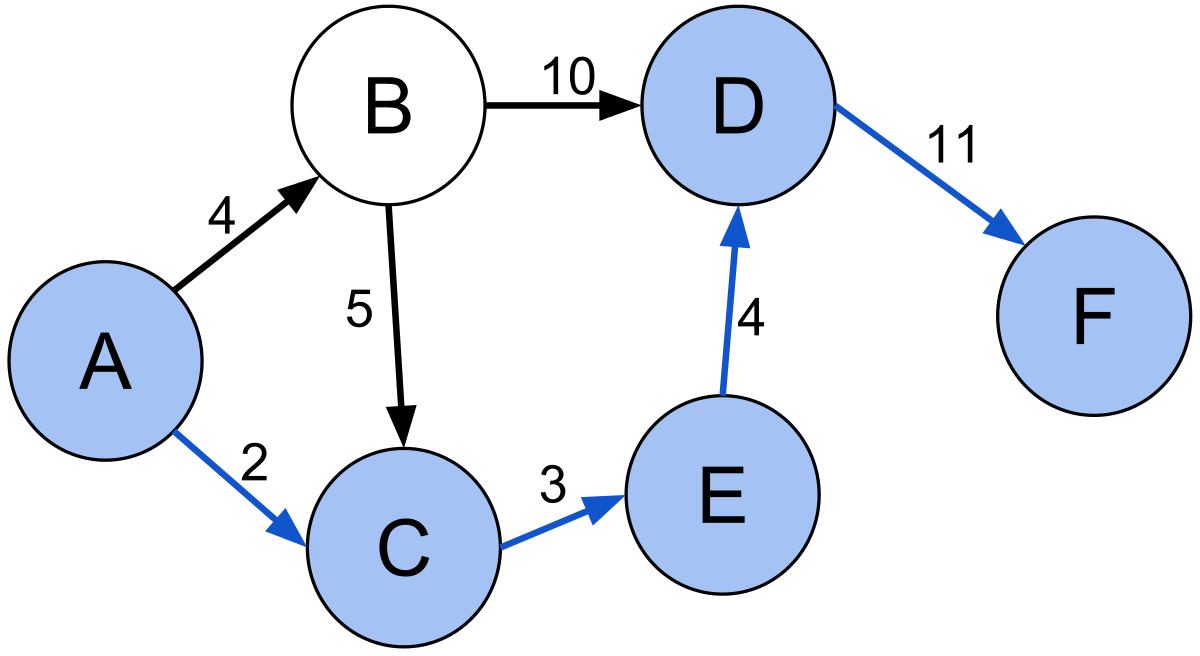
\includegraphics[width=0.5\textwidth]{ejemplo_camino_minimo.png}
    \caption*{El camino mínimo entre el par de vértices $A$ y $F$.}
\end{figure}

Este mínimo existe porque el conjunto de caminos es finito: a lo sumo hay $n!$, uno por cada permutación de los vértices de $G$. Esto no necesariamente vale en el caso de recorridos, que pueden tener vértices repetidos.

Un problema análogo es el de \textit{camino máximo}, que es el camino de peso máximo entre un par de vértices.

\subsection{Existencia}

A pesar de que un \textbf{camino} mínimo entre $u$ y $v$ siempre existen (asumiendo que están conectados), no es el caso para los recorridos: si un grafo tiene algún \textit{ciclo de peso negativo} (o simplemente \textit{ciclo negativo}) alcanzable desde $u$ y $v$, este puede ser transitado múltiples veces para obtener un peso tan bajo como se desee.

\subsection{Camino mínimo elemental}

El problema de esta índole más simple de definir (y más general) es el de \textit{camino mínimo elemental}:

\begin{problema}
    Dado un (di)grafo $G = (V, E, w)$ y un par de vértices $v, u \in V$, encontrar el camino (sin vértices repetidos) de peso mínimo.
\end{problema}

Como establecimos antes, este problema esta bien definido para cualquier grafo y cualquier par de vértices. El problema de \textit{camino máximo elemental}, donde se busca el camino de peso máximo, se puede reducir fácilmente a este: basta con tomar una función de peso $w'(e) = -w(e)$\footnote{A pesar de que los problemas son equivalentes, las aplicaciones de camino mínimo suelen ser en casos donde los pesos son no negativos (y por ende el grafo no tiene ciclos negativos). En tal caso, encontrar un camino máximo se vuelve más difícil, ya que negar los pesos hace que casi cualquier ciclo sea negativo. Es por esto que camino máximo se considera ``más difícil''.}.

Para el caso general, este problema es \hyperref[np-hard]{NP-hard}, así que se suelen estudiar casos restringidos. La restricción más importante para nuestros algoritmos es que el grafo no tenga ciclos negativos. En ese caso, encontrar un camino mínimo es equivalente a encontrar un recorrido mínimo.

\label{teorema-ciclos-negativos}
\begin{theorem*}
    Si un (di)grafo $G = (V, E, w)$ no tiene ningún ciclo negativo, existe un camino entre cualquier par de vértices $v, u \in V$ con peso total menor al de cualquier recorrido.
\end{theorem*}
\begin{proof}
    Supongamos que existe algún recorrido $R = v \cdots u$ que no es un camino y cuyo peso $w(R)$ es menor a la longitud de todos los caminos entre $v$ y $u$. Debido a que no es camino, tiene que pasar por dos veces por algún vértice $z$, definiendo un ciclo $R_{z_1 z_2}$\footnote{$z_1$ y $z_2$ no son vértices distintos, sino formas de distinguir las apariciones de $z$ en $R$.}. Como el grafo no tiene ciclos negativos, $w(P_{z_1 z_2}) \geq 0$, y entonces se puede definir un nuevo recorrido $R' = R_{v z_1} + R_{z_2 u}$ que ``recorta'' el ciclo, y cumple $w(R') = w(R) - w(R_{z_1 z_2}) \leq w(R)$. Este proceso puede repetirse hasta conseguir un camino de peso menor o igual al recorrido original, lo cual contradice la suposición inicial.
\end{proof}

\subsubsection{Subestructura óptima}

El problema de encontrar un camino mínimo $P_{uv}$ entre un par de vértices $u$ y $v$ cumple el \hyperref[optimalidad-bellman]{princpio de optimalidad de Bellman}: Cualquier subcamino $P_{u'v'} \subseteq P_{uv}$ es a su vez un camino mínimo entre $u'$ y $v'$.
\begin{theorem*}
    Dado un digrafo pesado $G = (V, E, w)$ sin ciclos negativos y un camino mínimo $P = v_1 \cdots v_k$, el subcamino $P_{v_i v_j}$ es un camino mínimo entre $v_i$ y $v_j$.
\end{theorem*}
\begin{proof}
    Supongamos que $P_{v_i v_j}$ no es un camino mínimo. Eso implica que existe un camino alternativo $P' = v_i \cdots v_j$ tal que $w(P') < w(P_{v_i v_j})$. En tal caso, se podría construir el recorrido $R = P_{v_1 v_i} + P' + P_{v_j v_k}$, para el cual existen dos posibilidades:
    \begin{itemize}
        \item Si el recorrido $R$ es un camino, entonces $w(R) = w(P_{v_1 v_i}) + w(P') + w(P_{v_j v_k}) < w(P_{v_1 v_i}) + w(P_{v_i v_j}) + w(P_{v_j v_k}) = w(P)$, lo cual es absurdo porque $P$ es un camino mínimo.
        \item Si el recorrido $R$ no es un camino, hay algún vértice $v_a$ por el que pasa 2 veces. Esto forma un ciclo $C = R_{v_{a1} v_{a2}}$ dentro del recorrido, que por hipótesis debe tener peso no negativo. Por lo tanto, si se ``recorta'' el ciclo, se obtiene un recorrido $R' = R_{v_1 v_{a1}} R_{v_{a2} v_k}$ de peso menor o igual. Estos recortes se pueden repetir hasta obtener un camino que, al igual que en el caso anterior, tiene peso estrictamente menor a $P$ (\textbf{Absurdo}).
    \end{itemize}

    Como ambas alternativas llevan a una contradicción, la suposición inicial ($P_{v_i v_j}$ no es camino mínimo) es falsa.
\end{proof}

\subsection{Árbol de caminos mínimos}

Ahora que definimos las restricciones necesarias (no hay ciclos negativos), se pueden empezar a analizar los métodos para encontrar caminos mínimos. Sorprendentemente, el problema de encontrar un camino mínimo entre $v$ y $u$ parece ser igual de difícil que el de encontrar el camino mínimo entre $v$ y todos los vértices del grafo, ya que no se conoce ningún algoritmo que resuelva el primero con una complejidad  de peor caso estrictamente menor a los métodos para resolver el otro.

Este nuevo problema se llama \textit{camino mínimo con un origen y múltiples destinos} (SSSP\footnote{\textit{Single Source Shortest Path.}}), y los caminos definen un árbol enraizado en $v$, llamado el \textit{árbol de caminos mínimos} (ACM). Un $v$-ACM es análogo a un árbol $v$-geodésico, solo que en este caso se cumple $\delta_T(v, u) = \delta_G(v, u)\ \forall u \in V$.

\section{Algoritmo de Dijkstra}

El \textit{algoritmo de Dijkstra} es uno de los más famosos en todo el área de computación. Este resuelve el problema de camino mínimo uno a todos, bajo la restricción de que los pesos de las aristas son no negativos.

\subsection{Definición}

El procedimiento general es similar al de Prim: se mantiene un árbol enraizado en el vértice inicial $v$ junto con una ``frontera'' de vértices adyacentes a los del árbol. En cada paso, se agrega el vértice de la frontera más cercano a la raíz. Esto puede ser clasificado como goloso, ya que en cada iteración se toma la decisión más ventajosa a corto plazo. Extendiendo la comparación, mientras que Prim agrega la arista segura de costo mínimo, Dijkstra agrega la que conecta al vértice con menor distancia a $v$.

\begin{codebox}
    \Procname{$\proc{Dijkstra}(G, w, s)$}
    \li $T \gets (V_T = \{s\}, E_T = \emptyset)$
    \li Inicializar arreglo $d$ con $+\infty$ en cada posición.
    \li $d[s] \gets 0$
    \li \For $i \gets 1$ \To $n - 1$ \Do
    \li $u \rightarrow v \gets \arg\min{\{d[x] + w(x \rightarrow y) \mid x \in V_T, y \in V - V_T\}}$
    \li $d[v] \gets d[u] + w(u \rightarrow v)$
    \li $V_T \gets V_T \cup \{v\}$
    \li $E_T \gets E_T \cup \{u \rightarrow v\}$
    \End
    \li \Return $(T, d)$
\end{codebox}

El diccionario $d$ contiene la distancia mínima entre $s$ y cada vértice. Esto se puede utilizar, entre otras cosas, para obtener el camino mínimo a cualquier vértice $u$ en tiempo lineal: se puede revisar el vecindario de entrada $N^-(u)$ hasta encontrar un vértice $v \in N^-(u)$ tal que $d[v] + w(v \rightarrow u) = d[u]$. Esto significa que hay un camino mínimo que pasa por la arista $v \rightarrow u$, y el proceso se puede repetir hasta llegar a $s$.

El algoritmo puede modificarse para grafos disconexos: debe mantener un conjunto de vértices conectados, y frenar cuando no quedan nuevos vértices por explorar. El comportamiento en ese caso es devolver los caminos mínimos a los vértices alcanzables (los demás están a distancia $\infty$).

\subsubsection{Generalización}

El procedimiento se puede generalizar para cualquier función $\bullet: \R \times \R \longrightarrow \R$ no decreciente de forma que el costo $w_\bullet(P)$ de un camino $P = v_1 \cdots v_k$ sea:
$$
    w_\bullet(v_1 \cdots v_k) =
    \begin{cases}
        0                                                    & \si k = 1 \\
        w_\bullet(v_1 \cdots v_{k-1}) \bullet c(v_{k-1} v_k) & \ecc
    \end{cases}
$$

La restricción de ser \textit{no decreciente} significa que $w_\bullet(P + y) \geq w_\bullet(P)$ para todo camino $P$ y vértice $y$. La suma cumple esto solo cuando los pesos son no negativos.

Si se define $\bullet$-peso de un camino $P$ al valor $w_\bullet(P)$, se puede llamar camino $\bullet$-mínimo al camino entre $v$ y $u$ con menor $\bullet$-peso (y $\delta_\bullet(v, u)$ al peso de ese camino). Más aún, el árbol de caminos $\bullet$-mínimos de $v$ es uno en el cual $\delta_{G,\bullet}(v, u) = \delta_{T, \bullet}(v, u)$ para todo $u$.

Finalmente, si se tiene un $\bullet$-ACM $T$ enraizado en $v$, se puede definir $w_\bullet(x \rightarrow v) = w_\bullet(P) \bullet w(x \rightarrow y)$, donde $P$ es el camino de $T$ entre $v$ y $x$. Esto permite diseñar el siguiente algoritmo general:

\begin{codebox}
    \Procname{$\proc{Dijkstra-$\bullet$}(G, w, s)$}
    \li $T \gets (V_T = \{s\}, E_T = \emptyset)$
    \li \For $i \gets 1$ \To $n - 1$ \Do
    \li $u \rightarrow v \gets \arg\min{\{w_\bullet(x \rightarrow y) \mid x \in V_T, y \in V - V_T\}}$
    \li $V_T \gets V_T \cup \{v\}$
    \li $E_T \gets E_T \cup \{u \rightarrow v\}$
    \End
    \li \Return $(T, d)$
\end{codebox}

Bajo esta definición, el algoritmo de Prim es solo una versión de \proc{Dijkstra-$\bullet$}, donde la función $\bullet(x, y)$ es $\max{\{x, y\}}$.

\subsection{Correctitud}

Se podría demostrar la correctitud de la función \proc{Dijkstra-$\bullet$}, pero para el final es más útil el caso particular de camino mínimo.

\begin{theorem*}
    Dado un (di)grafo pesado sin ciclos negativos $G = (V, E, w)$ y un origen $s \in V$, el algoritmo de Dijkstra devuelve un $s$-ACM $T$, y $d[u] = \delta(v, u)\ \forall u \in V$.
\end{theorem*}
\begin{proof}
    Se procede demostrando la siguiente hipótesis inductiva: para cada $0 \leq k \leq n - 1$, el grafo $T_k = (V_k, E_k)$ mantenido por Dijkstra en la $k$-ésima iteración es un árbol que cumple $\delta_{T_k}(s, u) = \delta_{G}(s, u)\ \forall u \in V_{k}$, y además $d[u] = \delta_{G}(s, u)\ \forall u \in V_{k}$.

    \textbf{Caso Base}: Antes de la primera iteración, $T_0 = (\{s\}, \emptyset)$, y se cumple que $d[s] = 0 = \delta(s, s)$ (por definición).

    \textbf{Paso Inductivo}: Llamemos $u \rightarrow v$ el arco que se agrega al árbol en la $k$-ésima iteración, es decir, $T_k = (V_k, E_k) = (V_{k - 1} \cup \{u\}, E_{k - 1} \cup \{u \rightarrow v\})$. Es claro que $T_k$ sigue siendo un árbol, ya que la nueva arista conecta a un vértice que no estaba en el grafo (y por ende no puede formar un ciclo).

    Sea $P = s \cdots y$ un camino mínimo entre $s$ e $y$, es decir, $w(P) = \delta(s, y)$. Tomamos el último vértice $x$ del camino que pertenece a $V_{k - 1}$, y sea $y$ el que lo sigue (estos deben existir, porque $x$ está en el conjunto, e $y$ no). Como se demostró anteriormente, $w(P_{su}) = \delta(s, u)$ (es subcamino de un camino mínimo). Como la arista $x \rightarrow y$ conecta un vértice de $V_{k - 1}$ con uno de $V - V_{k - 1}$, se debe cumplir que:
    \begin{flalign*}
         &  & d[u] + w(u \rightarrow v)         & \leq  d[x] + w(x \rightarrow y)        &  & \text{($u \rightarrow v$ fue elegida por Dijkstra)} \\
         &  & \delta(s, u) + w(u \rightarrow v) & \leq \delta(s, x) + w(x \rightarrow y) &  & \text{(Por HI, ya que $u, x \in T_{k - 1}$)}
    \end{flalign*}

    Entonces, se tiene que el camino une a $s$ con $v$ en $T_k$, $P'$ tiene un peso
    $$w(P') =
        \delta(s, u) + w(u \rightarrow v)
        \leq \delta(s, x) + w(x \rightarrow y)
        \underset{w \geq 0}{\leq} \underbrace{\delta(s, x) + w(x \rightarrow y) + w(P_{yv})}_{= w(P) \text{, que es un CM}}
        = \delta(s, v)$$

    Así que el camino $P'$ es mínimo, y $T_k$ cumple que las distancias de sus vértices son las mínimas en el grafo. Por otro lado, el nuevo valor de $d[v] = d[u] + w(u, v)$ es la distancia mínima de $s$ a $v$.

\end{proof}

\subsection{Complejidad}

La complejidad de Dijkstra es análoga a \hyperref[complejidad-prim]{la de Prim}: solo es necesario mantener un arreglo adicional con las distancias a cada nodo, lo cual no impone ningún costo en términos de tiempo. Por ende, el tiempo de ejecución dependerá de como se implemente la cola de prioridad de vértices a agregar:
\begin{itemize}
    \item \underline{Arreglo}: \BigO{|V|^2}.
    \item \underline{Binary Heap o AVL}: \BigO{|E|\log{|V|}}.
    \item \underline{Fibonacci Heap}: \BigO{|E| + |V|\log{|V|}}.
\end{itemize}

\section{Bellman-Ford}

El \textit{algoritmo de Bellman-Ford}, al igual que el de Dijkstra, resuelve el problema de camino mínimo de uno a todos. Sin embargo, a diferencia de este, Bellman-Ford puede ser utilizado en (di)grafos con pesos negativos (pero sin ciclos negativos). Si el grafo tiene algún ciclo alcanzable desde el vértice de origen, Bellman-Ford es capaz de detectarlo.

\subsection{Definición}

Este algoritmo se basa en ``\textit{relajar}'' las aristas del grafo. La relajación de $u \rightarrow v$ implica comprobar si el camino mínimo que va del origen a $v$ puede ser mejorado pasando por la arista. Si las distancias mínimas $\delta(s, v)$ se guardan en $d[v]$, se peude expresar de la siguiente manera:

\begin{codebox}
    \Procname{$\proc{Relajar}(u \rightarrow v, w)$}
    \li $d[v] \gets \min{\{d[u] + w(u \rightarrow v), d[v]\}}$
\end{codebox}

Bellman-Ford repite esta operación para cada arista, $|V| - 1$ veces. En cada iteración $i$ ciclo, los vértices se conectan a $s$ por caminos de a lo sumo $i$ aristas.

\begin{codebox}
    \Procname{$\proc{Bellman-Ford}(G, w, s)$}
    \li Inicializar arreglo de distancias $d$ con $+\infty$ en cada posición
    \li $d[s] \gets 0$
    \li \For $i \gets 0$ \To $n - 1$ \Do
    \li \For \Each $e \in E$ \Do
    \li $\proc{Relajar}(e, w)$
    \End
    \End
    \li \For \Each $u \rightarrow v \in E$ \Do
    \li \If $d[u] + w(u \rightarrow v) < d[v]$ \Then
    \li \Return Hay un ciclo negativo
    \End
    \End
    \li \Return $d$
\end{codebox}

El último ciclo chequea si existe algún ciclo negativo. Esto se debe a que, si alguna arista se puede relajar después de $i$ iteraciones, el recorrido más corto entre $s$ y algún vértice tiene $|V|$ aristas, lo cual implica que contiene un ciclo negativo (se demuestra más adelante).

El algoritmo puede adaptarse para devolver un $s$-ACM: basta con actualizar el padre de $v$ en \proc{Relajar}, es decir, asignar $prev[v] \gets u$.

\subsection{Correctitud}

Primero analizamos el caso de grafos sin ciclos negativos:

\begin{theorem*}
    Dado un (di)grafo pesado $G = (V, E, w)$ sin ciclos negativos, el algoritmo de Bellman-Ford devuelve en $d$ las distancias $d[v] = \delta(s, v)$.
\end{theorem*}
\begin{proof}
    Para demostrar esto, se demuestra la siguiente propiedad hipótesis inductiva: para cada iteración $k$ del ciclo exterior de Bellman-Ford, si un vértice $v$ está conectado a $s$ por un camino mínimo $P$ tal que $|P| \leq k$, se tiene que $d_{k}[v] = \delta(s, v)$, y $d_k[u] \geq \delta(s, u)\ \forall v \in V$.

    \textbf{Caso Base}: Para $k = 0$, el único vértice conectado por un camino de longitud $0$ es $s$, y se cumple que $d[s] = \delta(s, s) = 0$

    \textbf{Paso Inductivo}: Primero, demuestro la parte auxiliar de la hipótesis inductiva: sabiendo que $d_{k - 1}[u] \geq \delta(s, u)\ \forall v \in V$, se puede analizar la asignación de \proc{Relajar} (es el único procedimiento que cambia $d$ en el algoritmo):
    $$d_k[u] \gets \min{\{d_{k - 1}[u], d_{k - 1}[u'] + w(u' \rightarrow u)\}}$$

    Podemos ver que ambas opciones cumplen la propiedad: $d_{k - 1}[u] \geq \delta(s, u)$ por HI, mientras que: $d_{k - 1}[u'] + w(u' \rightarrow u) \geq \delta(s, u') + w(u' \rightarrow u) \geq \delta(s, u)$ (desigualdad triangular).

    Luego, por hipótesis sabemos que en el paso $k - 1$-ésimo se cumplía que $d_{k - 1}[v] = \delta(s, v)$ para cualquier vértice $v$ con camino mínimo de longitud menor o igual a $k - 1$. Esto se sigue cumpliendo en $d_k$ para esos mismos vértices gracias a que, como \proc{Relajar} asigna:
    $$d_k[v] \gets \min{\{d_{k - 1}[v], d_{k - 1}[u] + w(u \rightarrow v)\}}$$

    Se tiene que $d_k[v] \leq d_{k - 1}[v] = \delta(v, s)$. Como demostramos previamente, $d_k[v] \geq \delta(v, s)$, así que $d_k[v] = \delta(v, s)$.

    Por otro lado, para aquellos vértices $z$ tales que el camino mínimo de $s$ a $z$ es $P = s \cdots z$ de longitud $|P| = k$, sea $z'$ el anteúltimo vértice. Debido a que $P_{sz'} = s \cdots z'$ es también camino mínimo (es subcamino de un camino mínimo) y tiene longitud $k - 1$, sabemos por $HI$ que $d_{k - 1}[z'] = \delta(s, z')$. Esto, implica que $d_{k - 1}[z'] + w(z' \rightarrow z) = \delta(s, z') + w(z' \rightarrow z) = w(P) = \delta(s, z)$. Por lo tanto, en la asignación:
    $$d_k[z] \gets \min{\{d_{k - 1}[z], d_{k - 1}[z'] + w(z' \rightarrow z)\}}$$
    Como $d_{k - 1}[z] \geq \delta(s, z)$, se tiene $d_k = \delta(s, z)$.

    Finalmente, habiendo demostrado la inducción, nos sirve un caso particular de la misma: después de la última iteración, todos los vértices conectados al origen por un camino mínimo de longitud máxima $|V| - 1$ tendrán los pesos asignados de forma correcta. Estos son pesos son las distancias $\delta(s, v)$, porque en caso contrario el recorrido mínimo tendría que tener longitud mayor a $|V| - 1$, y por ende repetir algún vértice (esto \hyperref[teorema-ciclos-negativos]{no sucede} en grafos sin ciclos negativos).

\end{proof}

El comportamiento cuando hay ciclos negativos también es correcto:

\begin{theorem*}
    Si un (di)grafo pesado $G = (V, E, w)$ tiene algún ciclo de peso negativo $C$ alcanzable desde un origen $s$, el algoritmo de Bellman-Ford lo detecta.
\end{theorem*}
\begin{proof}
    Primero, demuestro la siguiente hipótesis inductiva: en la $k$-ésima iteración de relajaciones, cualquier vértice $u$ con distancia\footnote{Distancia es la longitud del camino más corto, no el peso del camino mínimo.} a $s$ menor o igual a $k$ cumple $d_k[v] < \infty$

    \textbf{Caso Base}: El único vértice alcanzable desde $s$ a través de $0$ aristas es $s$ en sí, y $d[s] = 0 < \infty$.

    \textbf{Paso inductivo}: Si la propiedad vale para $k - 1$, entonces $d_{k - 1}[u] < \infty$ para los $u$ a distancia $\leq k - 1$ de $s$. Después de la iteración $k$, eso se sigue cumpliendo para esos vértices, ya que \proc{Relajar} asigna un mínimo entre dos valores, uno de los cuales es $d_{k - 1}[u]$, así que $d_k[u] \leq d_{k - 1}[u] < \infty$.

    Por otro lado, si un vértice $u$ está a distancia $k$ de $s$, existe un camino $P = s \cdots u$ tal que $|P| = k$. Si llamamos $u'$ al anteúltimo vértice de $P$, se puede ver que $d_{k - 1}[u] < \infty$, ya que el camino $P_{su'}$ tiene longitud $k - 1$ (hipótesis inductiva). Luego, el valor $d_k[u]$ está dado por un mínimo entre dos valores, uno de los cuales es $d_{k - 1}[u'] + w(u' \rightarrow u) < \infty$ (es una suma de valores finitos), así que $d_k[u] < \infty$. Entonces, queda demostrado el caso $k$.

    En el caso particular de $k = |V| - 1$, cualquier vértice $v$ alcanzable desde $s$ tiene $d[v] < \infty$, ya que si existe un recorrido entre ambos, se pueden recortar los ciclos del mismo para obtener un camino (que tiene una longitud de a lo sumo $|V| - 1$).

    Sea $C = v_0 \cdots v_l$ el ciclo de peso negativo alcanzable desde $v$. Se tiene que:
    $$w(C) = \sum_{i = 1}^l w(v_{i - 1} \rightarrow v_i) < 0$$

    Supongamos que el algoritmo no detecta ningún ciclo. Esto implica que $d[u] + w(u \rightarrow v) < d[v]$ para todas las aristas del grafo. En particular, $d[v_i] \leq d[v_{i - 1}] + w(v_{i + 1} \rightarrow v_i)\ \forall i = 1 ... l$. Sumando estas desigualdades:
    \begin{align*}
        \sum_{i = 1}^l d[v_i] & \leq \sum_{i = 1}^l d[v_{i - 1}] + w(v_{i - 1} \rightarrow v_i)                \\
        \sum_{i = 1}^l d[v_i] & \leq \sum_{i = 1}^l d[v_{i - 1}] + \sum_{i = 1}^l w(v_{i - 1} \rightarrow v_i)
    \end{align*}

    Por otro lado, como $C$ es un ciclo, $v_0 = v_l$, y por ende:
    $$\sum_{i = 1}^k d[v_i] = \sum_{i = 0}^{k - 1} d[v_i] = \sum_{i = 1}^k d[v_{i - 1}]$$

    Como los vértices son alcanzables desde el origen, sus valores $d[v_i]$ son finitos, así que:
    \begin{align*}
        \sum_{i = 1}^l d[v_i]                               & \leq \sum_{i = 1}^l d[v_{i - 1}] + \sum_{i = 1}^l w(v_{i - 1} \rightarrow v_i) \\
        \sum_{i = 1}^l d[v_i] - \sum_{i = 1}^l d[v_{i - 1}] & \leq \sum_{i = 1}^l w(v_{i - 1} \rightarrow v_i)                               \\
        0                                                   & \leq \sum_{i = 1}^l w(v_{i - 1} \rightarrow v_i) = w(C)
    \end{align*}

    Esto es absurdo, así que el algoritmo tiene que haber detectado el ciclo.

\end{proof}

\subsection{Complejidad}

La complejidad de Bellman-Ford es fácil de calcular: \proc{Relajar} es una operación de tiempo constante, y corre $|E|$ veces en cada iteración (una por cada arista). Como hay $|V| - 1$ iteraciones, la complejidad es \BigO{|V||E|} (el último ciclo para comprobar la existencia de ciclos negativos es \BigO{|E|}, lo cual no cambia la complejidad).

\subsection{Mejoras}

% TODO

\subsection{Aplicación: Sistema de Restricciones de Diferencias}

Un problema que se puede resolver a través de Bellman-Ford es el de \textit{sistemas de restricciones de diferencias} (SRD). El enunciado es el siguiente:

\begin{problema}
    Encontrar un conjunto de valores $x_1, ..., x_n$, que respeten un sistema de $m$ inecuaciones de la forma:
    $$x_i - x_j \leq c_{ij}$$
\end{problema}

El problema se puede \hyperref[reducciones]{reducir} a camino mínimo el digrafo $D$, que tiene las siguiente características:
\begin{itemize}
    \item Para cada $i = 1, ..., n$, hay un vértice $v_i \in V_D$ que se corresponde con la incógnita $x_i$.
    \item Para cada inecuación $x_i - x_j \leq c_{ij}$, hay un arco $v_j \rightarrow v_i \in E_D$ de peso $w(v_j \rightarrow v_i) = c_{ij}$.
    \item Hay un vértice adicional $v_0$, que cuenta con arcos $v_0 \rightarrow v_i$ hacia todos los vértices $v_i$, todos de peso $w(v_0 \rightarrow v_i) = 0$.
\end{itemize}

El sistema tiene solución solo cuando el digrafo no tiene ciclos negativos

\begin{theorem*}
    Un sistema SRD tiene solución cuando el digrafo correspondiente $D$ no tiene ciclos negativos, y en tal caso la solución es $\{x_i = \delta(v_0, v_i) \mid 1 \leq i \leq n\}$.
\end{theorem*}
\begin{proof}
    Primero, veamos que pasa si $D$ tiene algún ciclo negativo $C = v_{i_0} \cdots v_{i_l}$. Supongamos que existe una solución $\{x_1, ..., x_n\}$. En tal caso, se tiene:
    $$\sum_{j = 1}^l w(v_{i_{j - 1}} \rightarrow v_{i_j}) = \sum_{j = 1}^l c_{i_j i_{j - 1}} < 0$$

    Si se suman las inecuaciones correspondientes del sistema, se llega a:
    \begin{align*}
        \underbrace{\sum_{j = 1}^l v_{i_j} - v_{i_{j - 1}}}_{\text{Suma telescópica}} & \leq \sum_{j = 1}^l c_{i_j i_{j - 1}} < 0 \\
        v_{i_l} - v_{i_0}                                                             & < 0
    \end{align*}

    Como $C$ es un ciclo, $v_{i_l} = v_{i_0}$, así que $0 < 0$ (\textbf{Absurdo}). Esto implica que no puede existir una solución para el sistema.

    Por otro lado, si no existe ningún ciclo de peso negativo, tomemos la asignación de valores $\{x_i = \delta(v_0, v_i) \mid 1 \leq i \leq n\}$. Entonces, para cada arco del grafo $v_j \rightarrow v_i$, se cumple la desigualdad triangular:
    $$\delta(v_0, v_i) \leq \delta(v_0, v_j) + w(v_j \rightarrow v_i)$$

    Reemplazando por los valores representados en el sistema,
    \begin{align*}
        x_i       & \leq x_j + c_{ij} \\
        x_i - x_j & \leq c_{ij}
    \end{align*}

    Es decir, se cumplen todas las desigualdades, así que $\{x_i = \delta(v_0, v_i) \mid 1 \leq i \leq n\}$ es una solución al sistema.

\end{proof}

Entonces, el sistema de ecuaciones se puede resolver encontrando el camino mínimo de un origen a todos los vértices o detectando algún ciclo de peso negativo alcanzable, que es precisamente lo que logra el algoritmo Bellman-Ford.

\section{Algoritmo de Floyd-Warshall}

\subsection{Definición}

El \textit{algoritmo de Floyd-Warshall} resuelve el problema de caminos mínimos todos a todos (APSP\footnote{All Pairs Shortest Paths}). Esto también se puede lograr corriendo alguno de los algoritmos anteriores (que devuelve el camino mínimo de uno a todos) para cada vértice, pero tendría desventajas: Dijkstra solo funciona cuando los pesos son no negativos, y $|V|$ ejecuciones  de Bellman-Ford sería (en general) más lento que este nuevo algoritmo. Al igual que antes, el grafo de entrada no puede tener ciclos de peso negativo.

Dado un grafo pesado $G = (V, E, w)$, se puede definir una matriz $L \in \R^{|V| \times |V|}$\footnote{Esto se puede considerar una extensión de la representación matriz de adyacencia, donde ahora cuando dos vértices están conectados por una arista se guarda su peso, y si no se guarda $\infty$.}, donde cada posición es el peso de la arista entre un par de vértices (si no existe una arista, el peso se considera infinito). Es decir,
$$
    l_{ij} =
    \begin{cases}
        0                      & \si i = j                     \\
        w(v_i \rightarrow v_j) & \si v_i \rightarrow v_j \in E \\
        \infty                 & \ecc
    \end{cases}
$$


El método calcula la \textit{matriz de distancias}, esto es, una matriz $D \in \R^{|V| \times |V|}$ tal que:
$$d_{ij} =
    \begin{cases}
        \delta(v_i, v_j) & \si \text{$v_i$ y $v_j$ están conectados} \\
        \infty           & \ecc
    \end{cases}$$

Para lograrlo, emplea la técnica de programación dinámica, empezando por $D^0 = L$, y calculando la siguiente matriz a través de la recurrencia:
$$d^k_{ij} = \min{\{d^{k - 1}_{ij}, d^{k - 1}_{ik} + d^{k - 1}_{kj}\}}$$

La matriz $D^k$ puede interpretarse como la matriz de distancias mínimas cuando se consideran solo los caminos que pasan por los vértices intermedios $\{v_1, ..., v_k\}$. Luego, después de $n$ iteraciones, la matriz $D^n$ es la matriz de distancias $D$.

El algoritmo se puede expresar de la siguiente manera:

\begin{codebox}
    \Procname{$\proc{Floyd-Warshall}(G)$}
    \li $D \gets L$
    \li \For $k = 1$ \To $|V|$ \Do
    \li \For $i = 1$ \To $|V|$ \Do
    \li \For $j = 1$ \To $|V|$ \Do
    \li $d_{ij} \gets \min{\{d_{ij}, d_{ik} + d_{kj}\}}$
    \End
    \End
    \End
    \li \Return $D$
\end{codebox}

En realidad, este algoritmo no implementa la recurrencia directamente: como utiliza una única matriz, hay casos en los que se asigna $d^k_{ij} = \min{\{d^{k - 1}_{ij}, d^k_{ik} + d^k_{kj}\}}$. Esto no afecta el resultado, solo tiene el efecto de converger más rápido a la matriz de distancias mínimas.

\subsection{Correctitud}

\begin{theorem*}
    Dado un (di)grafo pesado $G = (V, E, w)$ sin ciclos negativos, el algoritmo de Floyd-Warshall devuelve la matriz de distancias del mismo.
\end{theorem*}
\begin{proof}
    Para demostrar eso, primero demostramos por inducción que, en la iteración $k$ del ciclo exterior de FW, se cumple $d^k_{ij} = \delta(v_i, v_j)$ para cualquier par de vértices $v_i, v_j \in V$ conectados por un camino mínimo $P$ cuyos vértices intermedios están contenidos en $\{v_1, ..., v_k\}$ (es decir, $P \subseteq \{v_1, ..., v_k\} \cup \{v_i, v_j\}$). Además, se cumple para todos los vértices que $d^k_{ij} \geq \delta(v_i, v_j)$ (en todas las iteraciones).

    \textbf{Caso Base}: El caso base es $k = 0$. El conjunto de vértices intermedios sería $\emptyset$, y los únicos caminos mínimos sin vértices intermedios son aquellos constituidos por una sola arista. En esos casos, se cumple que $d^0_{ij} = w(v_i \rightarrow v_j) = \delta(v_i, v_j)$, gracias a que se asigna $D^0 \gets L$.

    Por otro lado, como asumimos que no hay ciclos de peso negativo, $\delta(v_i, v_i) = 0 = d^0_{ii} \forall i$, y para una arista $v_i \rightarrow v_j$ se tiene por desigualdad triangular:
    $$d^0_{ij} = w(v_i \rightarrow v_j) = \underbrace{{\delta(v_i, v_i)}}_{= 0} + w(v_i \rightarrow v_j) \geq \delta(v_i, v_j)$$

    \textbf{Paso Inductivo}: Supongamos que la propiedad vale en el caso $k - 1$. Recordemos que la asignación que se realiza en la iteración $k$ es:
    $$d^k_{ij} = \min{\{d^{k - 1}_{ij}, d^{k - 1}_{ik} + d^{k - 1}_{kj}\}}$$

    Para demostrar que $d^k_{ij} \geq \delta(v_i, v_j)$, notemos dos cosas:
    \begin{itemize}
        \item $d^{k - 1}_{ij} \geq \delta(v_i, v_j)$, por HI.
        \item $d^{k - 1}_{ik} + d^{k - 1}_{kj} \geq \delta(v_i, v_k) + \delta(v_k, v_j) \geq \delta(v_i, v_j)$, por HI y desigualdad triangular, respectivamente.
    \end{itemize}

    En todo caso, se cumple que $d^k_{ij} \geq \delta(v_i, v_j)$.

    Para los pares de vértices con caminos mínimos formados por vértices intermedios en el conjunto $\{v_1, ..., v_{k - 1}\}$, se sigue cumpliendo la propiedad, ya que la HI implica que $d^{k - 1}_{ij} = \delta(v_i, v_j)$ (así que $d^k_{ij} \leq \delta(v_i, v_j)$), y como recién demostramos que $d^k_{ij} \geq \delta(v_i, v_j)$, se tiene $d^k_{ij} = \delta(v_i, v_j)$.

    Por otro lado, sea $P = v_x \cdots v_y$ algún camino mínimo entre $v_x$ y $v_y$ que contiene al vértice $v_k$ y cuyos vértices intermedios están contenidos en $\{v_1, ..., v_k\}$. $P$ se puede descomponer como la concatenación $P_{v_x v_k} + P_{v_k v_y}$, y estos dos subcaminos (que son mínimos) están formados por vértices intermedios del conjunto $\{v_1, ..., v_{k - 1}\}$ (si estuviera $v_k$ en el medio, aparecería dos veces, y no serían caminos simples). Esto, por HI, implica que $d^{k - 1}_{xk} = \delta(v_x, v_k) = w(P_{v_x v_k})$ y $d^{k - 1}_{ky} = \delta(v_k, v_y) = w(P_{v_k v_y})$, así que cuando se asigna:
    $$d^k_{ij} = \min{\{d^{k - 1}_{ij}, d^{k - 1}_{ik} + d^{k - 1}_{kj}\}}$$

    Se obtiene $d^k_{xy} \leq d^{k - 1}_{xk} + d^{k - 1}_{ky} = w(P_{v_x v_k}) + w(P_{v_k v_y}) = w(P) = \delta(v_x, v_y)$ que, junto con $d^k_{xy} \geq \delta(v_x, v_y)$ (se demostró previamente), significa que $d^k_{xy} = \delta(v_x, v_y)$. Queda demostrado entonces que la propiedad vale para el caso $k$.

    Como, por inducción, la propiedad se cumple después de cualquier iteración $k$, se cumple en particular para después de la última, lo cual significa que todo par de vértices $v_i, v_j$ conectado por un camino mínimo con vértices intermedios en $\{1, ..., v_{|V|}\} = V$ cumple $d^k_{ij} = \delta(v_i, v_j)$. Esto incluye a cualquier par de vértices conectados, y para los vértices que no son alcanzables entre sí, la segunda propiedad garantiza que $d^k_{ij} \geq \delta(v_i, v_j) = \infty \implies d^k_{ij} = \infty$. Por ende, todas las distancias de $D^{|V|}$ son correctas.

\end{proof}

\subsection{Complejidad}

La complejidad de Floyd-Warshall es fácil de calcular: tiene 3 ciclos anidados, de $|V|$ iteraciones cada uno, en cuyo interior se realizan operaciones de tiempo constante, así que el algoritmo es \BigO{|V|^3}. Como se mencionó previamente, esto es mejor que correr $n$ veces Bellman-Ford, siempre que el grafo sea conexo (porque en ese caso $|E| \geq |V| - 1 \implies |E| \in \BigOmega{|V|}$).

Una posible mejora sería chequear en cada iteración si $d_{ii} < 0$ para algún $i$, ya que esto implica que el grafo tiene un ciclo negativo (en el teorema anterior se demuestra $d_{ii} \geq \delta(v_i, v_i) = 0$ cuando no hay ciclos negativos), y cortar la ejecución.

\section{Camino Mínimo en DAGs}

\subsection{Definición}

Para el caso de digrafos acíclicos, camino mínimo uno a muchos puede resolverse utilizando un algoritmo más eficiente que los anteriores. Este se basa en la siguiente fórmula para la distancia entre dos nodos:
$$
    \delta(u, v) =
    \begin{cases}
        0                                                             & \si u = v \\
        \min{\{\delta(u, z) + w(z \rightarrow v) \mid z \in N^-(v)\}} & \ecc
    \end{cases}
$$

Esto es intuitivo: la distancia mínima entre un par de nodos $u, v$ es el peso de algún camino mínimo $P = u \cdots v$. El anteúltimo vértice del camino $z$ está en el vecindario de entrada de $v$ (ya que tiene una arista que apunta hacia él), mientras que el subcamino $P_{uz}$ también es mínimo.

Esta relación no se puede utilizar para computar las distancias en un grafo con un ciclo $C = v \cdots v$, ya que la llamada $\delta(u, v)$ llevaría a un bucle de recursión infinita (porque existe un camino de $v$ a $v$ a través de los vecindarios de entrada).

\subsubsection{Versión Top-Down}

La fórmula se puede implementar como un algoritmo de programación dinámica top-down. Asumiendo que el arreglo de distancias (que funciona estructura de memoización) $D$ se inicializa con $\perp$ en todas las posiciones, el código es el siguiente:

\begin{codebox}
    \Procname{$\proc{SP-DAG-Top-Down}(G, s, v)$}
    \li \If $s == v$ \Then
    \li \Return $0$
    \End
    \li \If $D[v] ==\ \perp$ \Then
    \li $D[v] \gets \min{\{\proc{SP-DAG-Top-Down}(G, s, z) + w(z \rightarrow v) \mid z \in N^-(v)\}}$
    \End
    \li \Return $D[v]$
\end{codebox}

\subsubsection{Versión Bottom-Up}

Esto también se puede implementar de forma bottom-up: las distancias son calculadas en \hyperref[orden-topologico]{orden topológico}, lo cual asegura que $D[z]$ es calculado antes de $D[v]$ para cualquier $z \in N^-(v)$\footnote{Esto se debe a que, en un orden topológico, los vértices $v$ que son alcanzables desde $z$ aparecen después en la secuencia}.

\begin{codebox}
    \Procname{$\proc{SP-DAG-Bottom-Up}(G, s)$}
    \li Inicializar arreglo de distancias $D$.
    \li Calcular un orden topológico de $G$.
    \li \For \Each $v \in V$, en orden topológico \Do
    \li \If $s == v$ \Then
    \li $D[v] \gets 0$
    \li \Else
    \li \If $N^-(v) \neq \emptyset$ \Then
    \li $D[v] \gets \min{\{D[z] + w(z \rightarrow v) \mid z \in N^-(v)\}}$
    \li \Else 
    \li $D[v] \gets \infty$
    \End
    \li \Return $D$
\end{codebox}

\subsection{Complejidad}

Ambos métodos tienen una complejidad \BigO{|V| + |E|} ya que pasan $1$ vez por cada nodo $v$, realizando una operación \BigO{d^-(v)}. En el caso bottom-up, se realiza el paso adicional de computar un orden topológico, pero esto también se puede realizar en tiempo lineal a través de DFS.

\section{Algoritmo de Johnson}

\subsection{Definición}

El algoritmo de Johnson resuelve el problema de camino mínimo todos a todos. Es una alternativa al algoritmo de Floyd-Warshall, y es más eficiente para grafos ralos. La idea general del método es ``repesar'' las aristas del grafo, de forma que todos los pesos nuevos sean no negativos y se preserven los caminos mínimos, para luego aplicar el algoritmo de Dijkstra en cada nodo.

El proceso de repesar se basa en el siguiente teorema:

\begin{theorem*}
    Dado un (di)grafo pesado $G = (V, E, w)$ y una función $h: V \longrightarrow \R$, se puede definir una nueva función de peso:
    $$\hat{w}(u \rightarrow v) = w(u \rightarrow v) + h(u) - h(v)$$

    Luego, si se toma el grafo ``repesado'' $\hat{G} = (V, E, \hat{w})$, cualquier camino mínimo $P$ en $G$ sigue siendo mínimo en $\hat{G}$, y $G$ tiene un ciclo negativo $\iff$ $\hat{G}$ tiene un ciclo negativo.
\end{theorem*}
\begin{proof}
    Dado un recorrido cualquiera $P = \langle v_0, ..., v_k \rangle$ se puede ver que:
    \begin{align*}
        \hat{w}(P) & = \sum_{i=1}^k \hat{w}(v_{i - 1}, v_i)                                                                       \\
                   & = \sum_{i=1}^k w(v_{i - 1}, v_i) + h(v_{i - 1}) - h(v_i)                                                     \\
                   & = \sum_{i=1}^k w(v_{i - 1}, v_i) + \underbrace{\sum_{i=1}^k h(v_{i - 1}) - h(v_i)}_{\text{Suma telescópica}} \\
                   & = \sum_{i=1}^k w(v_{i - 1}, v_i) + h(v_0) - h(v_k)                                                           \\
                   & = w(P) + h(v_0) - h(v_k)
    \end{align*}

    Por ende, si $P'$ es un camino mínimo entre $u$ y $v$ en $G$, se tiene:
    \begin{flalign*}
         &  & w(P')                & \leq w(P)               &  & \forall P \text{ camino entre $u$ y $v$} \\
         &  & w(P')  + h(u) - h(v) & \leq w(P) + h(u) - h(v) &  & \forall P \text{ camino entre $u$ y $v$} \\
         &  & \hat{w}(P')          & \leq \hat{w}(P)         &  & \forall P \text{ camino entre $u$ y $v$}
    \end{flalign*}

    Entonces, $P'$ sigue siendo camino mínimo en $\hat{G}$.

    Por otro lado, dado un ciclo $C = u \cdots u$, su peso en $\hat{G}$ es $\hat{w}(C) = w(C) + h(u) - h(u) = w(C)$, así que $\hat{G}$ tiene ciclos negativos si y solo si $G$ los tiene.

\end{proof}

Para aprovechar este resultado, hace falta encontrar una función $h: V \longrightarrow \R$ que permita asignar valores no negativos a todos los pesos. El algoritmo de Johnson logra esto agregando un vértice adicional $s$ a $G$, conectado a todos los vértices con aristas de peso $0$, y calculando las distancias mínimas de $s$ a los demás (a través del algoritmo de Bellman-Ford, acá es donde el procedimiento falla si hay un ciclo negativo). Luego, toma $h(v) = \delta(s, v)$, que resulta en pesos no negativos ya que:
\begin{flalign*}
     &  & \delta(s, v) & \leq \delta(s, u) + w(u \rightarrow v) &  & \text{(Desigualdad triangular)} \\
     &  & h(v)         & \leq h(u) + w(u \rightarrow v)         &  &                                 \\
     &  & 0            & \leq w(u \rightarrow v) + h(u) - h(v)  &  &                                 \\
     &  & 0            & \leq \hat{w}(u \rightarrow v)          &  &
\end{flalign*}

Luego, se puede correr Dijkstra en cada vértice para obtener las distancias de todos a todos. El código es el siguiente:

\begin{codebox}
    \Procname{$\proc{Johnson}(G, w)$}
    \li $G' \gets (V \cup \{s\}, E \cup \{s \rightarrow v \mid s \in E\})$, $w(s, v) = 0\ \forall v \in V$
    \li \If $\proc{Bellman-Ford}(G', w, s)$ encuentra un ciclo negativo \Then
    \li \Return Hay un ciclo negativo
    \li \Else \proc{Bellman-Ford} devolvió las distancias $\delta(s, v)\ \forall v \in V$.
    \li Definir $\hat{w}(u \rightarrow v) \gets w(u \rightarrow v) + \delta(s, u) - \delta(s, v)\ \forall u \rightarrow v \in E$.
    \li Inicializar matriz $D \in \R^{|V| \times |V|}$
    \li \For \Each $u \in V$ \Do
    \li Correr $\proc{Dijkstra}(G, \hat{w}, u)$ para obtener $\hat{\delta}(u, v)\ \forall v \in V$
    \li Asignar $d_{uv} \gets \hat{\delta}(u, v) - \delta(s, v) + \delta(s, u)\ \forall v \in V$
    \End
    \li \Return $D$
    \End
\end{codebox}

\subsection{Complejidad}

La ejecución del algoritmo de Johnson se divide en dos partes. Primero, se ejecuta Bellman-Ford en el vértice agregado $s$, lo cual tiene una complejidad de \BigO{|V||E|}. Luego, se corre el algoritmo de Dijkstra una vez en cada vértice, y el tiempo de ejeución de eso depende de la cola de prioridad que utilice ese procedimiento. Si se utiliza un Fibonacci heap, la complejidad de Dijkstra es \BigO{|V|\log{|V|} + |E|}, así que la complejidad total de Johnson es \BigO{|V|^2\log{|V|} + |V||E|}.


\chapter{Flujo en Redes}
\label{flujo}

\section{Flujo máximo}

Una \textit{red de flujo} es un digrafo $N = (V, E)$ junto con una función de \textit{capacidad} $u: E \longrightarrow \Z_+$ y un par de nodos $s, t \in V$, llamados origen y destino. Un \textit{flujo factible} $x: E \longrightarrow \Z_+$ en esa red es una asignación de valores a las aristas, de forma que se cumpla:
\begin{itemize}
    \item $0 \leq x(v_i \rightarrow v_j) \leq u(v_i \rightarrow v_j)$ (Respeta las capacidades).
    \item $\forall v_i \in V - \{s, t\},$
          \begin{flalign*}
               &  & \sum_{u \in N^+(v)} x(u \rightarrow v) = \sum_{u \in N^-(v)} x(v \rightarrow u) &  & \textit{(Conservación)}
          \end{flalign*}
\end{itemize}


El \textit{valor del flujo} $x$ es la cantidad neta que sale del vértice $s$, es decir:
$$F = \sum_{u \in N^+(s)} x(u \rightarrow s) - \sum_{u \in N^-(s)} x(s \rightarrow u)$$

Entonces, se puede definir el problema de flujo máximo:

\begin{problema}
    Dada una red de flujo $N = (V, E, u)$ con origen $s$ y destino $t$, encontrar un flujo factible $x$ que tenga valor $F$ máximo. Es decir, maximizar:
    $$F = \sum_{u \in N^+(v)} x(u \rightarrow s) - \sum_{u \in N^-(v)} x(s \rightarrow u)$$

    Sujeto a:
    \begin{itemize}
        \item $0 \leq x(e) \leq u(e)\ \forall e \in E$
        \item $\forall v_i \in V - \{s, t\},$
              $$\sum_{u \in N^+(v)} x(u \rightarrow v) = \sum_{u \in N^-(v)} x(v \rightarrow u)$$
    \end{itemize}
\end{problema}

Las unidades del flujo se pueden considerar ``paquetes'' que viajan del origen $s$ al destino $t$, donde cada paquete puede tomar cualquier ruta que tenga la capacidad necesaria.

\subsection{Corte}

Un \textit{corte} en una red de flujo $N = (V, E, u)$ es un subconjunto $S \subseteq V$ tal que $s \in S$ y $t \notin S$. Por otro lado, dado un par de subconjuntos $S, T \subseteq V$, se define:
$$ST = \{u \rightarrow v \mid u \rightarrow v \in E, u \in S, v \in T\}$$

\begin{theorem*}
    \leavevmode

    Sea $x$ un flujo definido en una red $N = (V, E, u)$ y sea $S$ un corte. Entonces:
    $$F = \sum_{e \in S\bar{S}} x(e) - \sum_{e \in \bar{S}S} x(e)$$

    Donde $\bar{S} = V - S$.
\end{theorem*}
\begin{proof}
    Sumando los flujos netos que pasan por los vértices de $S$, se obtiene:
    $$\sum_{v \in S}\underbrace{\left(\sum_{u \in N^+(v)} x(u \rightarrow v) - \sum_{u \in N^-(v)} x(v \rightarrow u)\right)}_{\text{Siempre $0$, excepto para $v = s$}} = F + 0$$

    Por otro lado, los términos de la sumatoria representan todas las aristas que conectan un nodo de $S$ con uno de $V$, así que:
    $$F = \sum_{e \in SV} x(e) - \sum_{e \in VS} x(e)$$

    Las aristas de $SS$ aparecen en ambas sumatorias, así que se cancelan. Los únicos términos que quedan los las aristas que están en $S(V - S) = S\bar{S}$:

    $$F = \sum_{e \in S\bar{S}} x(e) - \sum_{e \in \bar{S}S} x(e)$$

\end{proof}

Por otro lado, la capacidad de un corte $S$ es la cantidad de flujo que puede salir del mismo, es decir:
$$u(S) = \sum_{e \in S\bar{S}} u(e)$$

Luego, se puede definir otro problema de flujo, el de corte mínimo:

\begin{problema}
    Dada una red de flujo $N = (V, E, u)$ con origen $s$ y destino $t$, encontrar el corte $S$ con capacidad mínima.
\end{problema}

A partir del último teorema, se puede ver que:
$$F = \sum_{e \in S\bar{S}} \underbrace{x(e)}_{\leq u(e)} - \sum_{e \in \bar{S}S} \underbrace{x(e)}_{\geq 0} \leq u(S)$$

Esto vale para cualquier valor de flujo $F$, y cualquier corte $S$. Esto es intuitivo: como las unidades de flujos empiezan en el origen $s$, todas deben pasar por alguna arista de $S\bar{S}$ para llegar al destino $t$.

\subsection{Certificado de optimalidad}
\label{flujo-certificado-optimalidad}

Un \textit{certificado de optimalidad} para una instancia de un problema de optimización es un valor que permite verificar que la solución una solución dada es efectivamente óptima (y, generalmente, hacerlo en menor tiempo que el que toma resolver el problema). El flujo máximo cuenta con uno: si se encuentra un flujo factible $x^*$ y un corte $S^*$ tales que $F^* = u(S)$, se tiene que, para cualquier valor de flujo $F$,
$$F \leq u(S) = F^*$$

Así que $x^*$ es un flujo máximo.

\subsection{Red residual y camino de aumento}

Dada una red de flujo $N = (V, E, u)$ y un flujo factible $x$, la \textit{red residual} $R(N, x) = (V, E_R)$ es un digrafo\footnote{En realidad, $R(N, x)$ es un multigrafo, debido a que cuando $N$ contiene aristas $v_i \rightarrow v_j$ y $v_j \rightarrow v_i$, y estas cumplen $0 < x(e) < u(e)$, la red residual tiene 4 aristas entre $v_i$ y $v_j$.} definido por:
\begin{itemize}
    \item $x(v \rightarrow w) < u(v \rightarrow w) \iff v \rightarrow w \in E_R$
    \item $x(v \rightarrow w) > 0 \iff w \rightarrow v \in E_R$
\end{itemize}

Además, se puede definir la \textit{capacidad residual} de una arista de $R(N, x)$ de la siguiente manera:
$$
    \Delta(v \rightarrow w) =
    \begin{cases}
        u(v \rightarrow w) - x(v \rightarrow w) & \si v \rightarrow w \in E \\
        x(v \rightarrow w)                      & \ecc
    \end{cases}
$$

Luego, un \textit{camino de aumento} es un camino orientado en el grafo $R(N, x)$ que va de $s$ a $t$. Para un camino $P$ se define $\Delta(P) = \min_{e \in P}{\{\Delta(e)\}}$.

\label{teorema-camino-aumento}
\begin{theorem*}
    Dada una red de flujo $N = (V, E, u)$ junto con un flujo factible $x$, si $P$ es un camino entre $s$ y $t$ en la red residual $R(N, x)$, se puede definir un nuevo flujo $\bar{x}$:
    $$
        \bar{x}(v \rightarrow w) =
        \begin{cases}
            x(v \rightarrow w) + \Delta(P) & \si v \rightarrow w \in P \\
            x(w \rightarrow v) - \Delta(P) & \si w \rightarrow v \in P \\
            x(v \rightarrow w)             & \ecc
        \end{cases}
    $$

    Luego, $\bar{x}$ es un flujo factible, y tiene un valor $\bar{F} = F + \Delta(P)$.
\end{theorem*}
\begin{proof}
    Para facilitar la demostración, introduzco una notación no estándar: si $e = u \rightarrow v$, $e^T := v \rightarrow u$.

    Primero, verifiquemos que $\bar{x}$ es un flujo factible.
    \begin{itemize}
        \item \textbf{Respeta las capacidades}: Solo hace falta verificar las capacidades de las aristas de $P$, ya que el flujo que pasa por las demás no se modifica (y $\bar{x}$ es un flujo factible). Entonces, veamos que pasa para las aristas $e \in P$.

              Si $e \in E$, entonces $x(e) < u(e)$ (ya que la arista también está en la red residual). Además, por la definición de $\Delta(P)$, se tiene que:
              $$\Delta(P) \leq \Delta(e) = u(e) - x(e)$$

              Esto implica que el nuevo flujo de la arista respeta la capacidad:
              $$\bar{x}(e) = x(e) + \Delta(P) \leq x(e) + u(e) - x(e) = u(e)$$

              Por otro lado, si $e^T \in E$, eso implica que $x(e^T) > 0$ (ya que la arista inversa está en la red residual). En cuanto a la capacidad residual de la arista,
              $$\Delta(P) \leq \Delta(e) = x(e^T)$$

              Entonces, el nuevo flujo es no negativo:
              $$\bar{x}(e^T) = x(e^T) - \Delta(P) \geq x(e^T) - x(e^T) = 0$$

        \item \textbf{Respeta la conservación}: De nuevo, para vértices por los que no pasa el camino, el flujo no cambia, así que la conservación se mantiene.

              Para cada vértice $v \in P - \{s, t\}$, sean $e_1 = a \rightarrow v$ y $e_2 = v \rightarrow b$ las dos\footnote{Son dos aristas porque, por ser camino, no se pasa dos veces por $v$.} aristas de $P$ que contienen a $v$. Observemos que el flujo neto que pasa por $v$ es:
              $$\sum_{e \in N^+(v)} \bar{x}(e) - \sum_{e \in N^-(v)} \bar{x}(e)$$

              Para los valores de flujo de $e_1, e_2$, existen 4 posibilidades:
              \begin{enumerate}
                  \item $e_1, e_2 \in E$: el flujo neto es:
                        \begin{align*}
                            \sum_{e \in N^+(v)} \bar{x}(e) - \sum_{e \in N^-(v)} \bar{x}(e) = \sum_{e \in N^+(v) - \{e_1\}} x(e) - \sum_{e \in N^-(v) - \{e_2\}} x(e) + \bar{x}(e_1) - \bar{x}(e_2) \\
                            = \sum_{e \in N^+(v) - \{e_1\}} x(e) - \sum_{e \in N^-(v) - \{e_2\}} x(e) + x(e_1) + \Delta(P) - x(e_2) - \Delta(P)                                                     \\
                            = \sum_{e \in N^+(v)} x(e) - \sum_{e \in N^-(v)} x(e) = 0
                        \end{align*}
                        % TODO: los otros casos
                  \item $e_1^T, e_2^T \in E$:
                  \item $e_1, e_2^T \in E$:
                  \item $e_1^T, e_2 \in E$:
              \end{enumerate}
    \end{itemize}

    Por otro lado, para calcular el valor del nuevo flujo, vamos a asumir que el vértice $s$ no tiene aristas entrantes ($d^-(s) = 0$). Esto es razonable: si hay flujo entrante a $s$, se forma un ciclo que se puede ``cancelar'', así que no es necesario modelarlo. Bajo esta suposición, el valor del flujo $\bar{x}$ es:
    $$\bar{F} = \sum_{w \in N^-(s)} x(w \rightarrow s) - \sum_{w \in N^+(s)} x(s \rightarrow w)$$
\end{proof}

\section{Método de Ford-Fulkerson}

El \textit{método de Ford-Fulkerson} es un esquema para resolver el problema de flujo máximo en una red de flujo basado en encontrar caminos de aumento dentro de la red residual. Esto funciona gracias al siguiente teorema:

\begin{theorem*}
    Sea $N = (V, E, u)$ una red de flujo y $x$ un flujo factible en esa red. Luego, $x$ es un flujo máximo $\iff$ no existe camino de aumento en $R(G, x)$.
\end{theorem*}
\begin{proof}
    \leavevmode

    $\implies$) Se demuestra el contrarrecíproco: por el teorema anterior, si existe un camino de aumento $P$, se puede definir el flujo $\bar{x}$ que tiene como valor $\bar{F} = F + \Delta(P)$. Como $\Delta(P) = \min_{e \in P}{\{\Delta(e)\}}$ y, por definición $\Delta(e) > 0\ \forall e \in E_R$, se tiene que $\Delta(P) > 0$, así que $\bar{F} > F$. Por lo tanto, $x$ no es un flujo máximo.

    $\impliedby$) Supongamos que no existe camino de aumento en $R(G, x)$. Entonces, sea $S$ el corte que contiene a todos los vértices alcanzables desde $s$ en la red residual (es un corte porque, si contuviera a $t$, habría un camino de aumento). Entonces, si se consideran las aristas $v \rightarrow w \in S\bar{S}$, sabemos que $v \rightarrow w \notin E_R$, así que $x(v \rightarrow w) = u(v \rightarrow w)$. Además, para las aristas $v' \rightarrow w' \in S\bar{S}$, también sabemos que $w' \rightarrow v \notin E_R$, así que $x(v' \rightarrow w') = 0$. Por ende, se tiene:
    $$F = \sum_{e \in S\bar{S}} x(e) - \sum_{e \in \bar{S}S} x(e) = \sum_{e \in S\bar{S}} u(e) - 0 = u(S)$$

    Como se demostró \hyperref[flujo-certificado-optimalidad]{anteriormente}, si se encuentra un flujo $x$ de valor $F$ y un corte $S$ tal que $F = u(S)$, el flujo es máximo y el corte mínimo.

\end{proof}

Por ende, si se incrementa el flujo a través de caminos de aumento hasta que la red residual no tenga más, se llega a un flujo máximo. El esquema es el siguiente:

\begin{codebox}
    \Procname{$\proc{Ford-Fulkerson}(N = (V, E, u))$}
        \li Inicializar flujo inicial $x$ con $x(e)\ \forall e \in E$.
        \li \While $\exists P$ camino de aumento en $R(N, x)$ \Do
        \li \For \Each $(v \rightarrow w) \in P$ \Do
        \li \If $(v \rightarrow w) \in E$ \Then
        \li $x(v \rightarrow w) \gets x(v \rightarrow w) + \Delta(P)$
        \li \Else
        \li $x(w \rightarrow v) \gets x(w \rightarrow v) - \Delta(P)$
        \End
        \End
        \End
        \li \Return $x$
\end{codebox}

Ford-Fulkerson se denomina un esquema, y no un algoritmo\footnote{A veces sí se lo llama algoritmo, y en ese caso no se especifica el camino que se elige.}, porque el criterio con el cuál encuentra el camino de aumento $P$ en cada iteración no se especifica. Existen algoritmos que implementan este esquema con una elección particular de camino de aumento, como el de \hyperref[edmonds-karp]{Edmonds-Karp}.

\subsection{Complejidad}
Para analizar la complejidad del esquema de Ford-Fulkerson, es necesario acotar la cantidad de iteraciones que hace el ciclo exterior. Para ello, nos valemos del siguiente teorema:

\begin{theorem*}
    Si las capacidades de una red $N = (V, E, u)$ cumplen $u(e) \in \Z$, el flujo máximo de $N$ tiene también valores enteros, y el esquema de \textit{Ford-Fulkerson} puede encontrar siempre un camino de aumento $P$ con $\Delta(P) \in \Z$.
\end{theorem*}
\begin{proof}
    Se puede demostrar haciendo inducción en las iteraciones de F\&F: en el paso $k$-ésimo, el flujo $x_k$ tiene valores enteros, y se puede encontrar un camino de aumento con valor entero.

    \textbf{Caso Base}: En el paso $0$, el flujo $x$ vale $x(e) = 0 \in \Z$ para todas las aristas $e$.

    \textbf{Paso Inductivo}: Asumiendo que en el paso $k - 1$-ésimo vale la propiedad, se tiene que $x_{k - 1}(e) \in \Z\ \forall e \in E$. Sabemos que si hay algún camino de aumento $P$, su valor $\Delta(P)$ se define como:
    $$\Delta(P) = \min{\{\Delta(e) \mid e \in P\}}$$

    Luego, como $\Delta(e) \in \{u(e) - x_{k - 1}(e), x_{k - 1}(e)\} \subseteq \Z$, se tiene que $\Delta(P) \in \Z$. Esto además implica que $x_k$ tiene valores enteros, porque $x_k$ se define como:
    $$
        x_k(v \rightarrow w) =
        \begin{cases}
            x_{k - 1}(v \rightarrow w) + \Delta(P) & \si v \rightarrow w \in P \\
            x_{k - 1}(w \rightarrow v) - \Delta(P) & \si w \rightarrow v \in P \\
            x_{k - 1}(v \rightarrow w)             & \ecc
        \end{cases}$$

    En todos los casos, los valores son enteros, así que la propiedad vale para el caso $k$.

\end{proof}

A partir de este teorema se puede ver que, cuando las capacidades son enteros, el esquema de F\&F realiza como máximo $F$ iteraciones: en cada paso, se encuentra un camino de aumento $P$ que cumple $\Delta(P) \geq 0 \land \Delta(P) \in \Z \implies \Delta(P) \geq 1$, así que en a lo sumo $F$ pasos se llega a un flujo de valor $F$. Esto implica que la complejidad total del algoritmo es \BigO{|V|F}, porque en cada iteración se realiza una operación constante para cada vértice del camino $P$ (que puede contener a todos los vértices).

Para expresar la complejidad sin saber el flujo máximo, se pueden encontrar cotas superiores para el mismo, como la suma de las capacidades $\sum_{e \in E} u(E)$, o el máximo $\max{\{u(e) \mid e \in E\}}$.

\subsection{Algoritmo de Edmonds-Karp}
\label{edmonds-karp}

El \textit{algoritmo de Edmonds-Karp} es una versión del de Ford-Fulkerson. En este caso, el camino de aumento es encontrado a través de BFS. Esto permite asegurar una cota de \BigO{|V||E|^2}.

\section{Matching Máximo en Grafo Bipartitos}

\subsection{Definición}

Dado un grafo bipartito $G = (V, E)$ con bipartición $(V_1, V_2)$, un \textit{matching} $M \subseteq E$ es un conjunto de aristas tal que:
$$\forall u \rightarrow v \in M,\ (u \in V_1 \land v \in V_2) \lor (u \in V_2 \land v \in V_1)$$

Otra definición equivalente para $M$ sería que cualquier vértice $v \in V$ es incidente a a lo sumo 1 arista de $M$. El problema de matching máximo en grafos bipartitos es:

\begin{problema}
    Dado grafo bipartito $G = (V, E)$, encontrar el matching $M^*$ de cardinal máximo. Es decir,
    $$M^* = \arg\max{\{\#M \mid M \text{ es matching en } G\}}$$
\end{problema}

Este problema se puede resolver reduciéndolo a flujo máximo.

\subsection{Solución}

Para resolver matching máximo en el grafo bipartito $G = (V, E)$, se puede definir la red de flujo $N =(V', E', u)$ de la siguiente forma:
\begin{itemize}
    \item $V' = V \cup \{s, t\}$
    \item $E' = E \cup \{s \rightarrow v \mid v \in V_1\} \cup \{w \rightarrow t \mid w \in V_2\}$
    \item $u(e) = 1\ \forall e \in E'$
\end{itemize}

Luego, el flujo máximo de la red pasará por un conjunto de aristas que conforman un matching $M$ de cardinal máximo.

% TODO: Demostrar

\section{Flujo de costo mínimo}

\begin{problema}
    Dada una red de flujo $N = (V, E, u)$ que tiene además:
    \begin{itemize}
        \item Una función de costo unitario (por cada unidad de flujo) en cada arista $c: E \rightarrow \Z_+$.
        \item Un \textit{imbalance} para cada nodo $b: V \rightarrow \Z_+$.
    \end{itemize}

    Encontrar el \textit{flujo de costo mínimo} $x: E \rightarrow \Z_+$, esto es, un flujo que:
    \begin{itemize}
        \item Respeta el imbalance de cada nodo $v \in V$:
              $$b(v) = \sum_{w \in N^+(v)} x(v \rightarrow w) - \sum_{w \in N^-(v)} x(w \rightarrow v)$$
        \item Respeta las capacidades de las aristas $e \in E$:
              $$0 \leq x(e) \leq u(e)$$
        \item Tiene costo $T = \sum_{e \in E} c(e) \cdot x(e)$ es mínimo.
    \end{itemize}
\end{problema}

En este caso, vamos a asumir que los valores son enteros, y que los imbalances se balancean ($\sum_{v \in V} b(v) = 0$).

Cuando los imbalances son todos nulos, el flujo se denomina una \textit{circulación}. Las circulaciones cumplen la siguiente propiedad:

\begin{theorem*}
    Dada una red de flujo $N = (V, E, u)$, una circulación $x$ puede ser descompuesta en combinación de circulaciones $x_1, ..., x_k$ tal que:
    $$x(e) = \sum_{i = 1}^k x_i(e)$$

    Y cada circulación $x_i$ está compuesta por un único ciclo $C$ (por el resto de las aristas $e' \in E - C$, el flujo $x_i(e) = 0$).
\end{theorem*}
\begin{proof}
    Esto se puede demostrar de forma constructiva: tomemos un nodo cualquiera $v$ que sea cola de un arco con flujo no nulo. Como no hay imbalances en la red, es claro que $v$ tiene que ser parte de un ciclo con flujo positivo: si no, se podría tomar un camino $P$ maximal que se extiende a izquierda y derecha por aristas de flujo positivo. Si no se forma un ciclo, el vértice al principio del camino tendría flujo neto positivo, y el del final flujo neto negativo.

    Sabiendo que $v$ forma parte de algún ciclo $C$ compuesto por aristas con flujo no nulo, se puede definir $\Delta(C) = \min{\{x(e) \mid e \in C\}}$. Luego, podemos tomar un flujo alternativo $\bar{x}$ definido como
    $$
        \bar{x}(e) =
        \begin{cases}
            x(e) - \Delta(C) & \si e \in C \\
            x(e)             & \ecc
        \end{cases}
    $$

    El flujo que pasa por los nodos fuera de $C$ no se ve afectado, mientras que los que están en el ciclo mantienen la conservación, ya que cada $\Delta(C)$ unidades que pierden por una arista de entrada son compensadas por una pérdida equivalente en una arista de salida. Esto significa que $\bar{x}$ es una circulación válida, y además sabemos que el flujo que pasa por las aristas de $C$ es estrictamente menor.

    El proceso anterior puede repetirse hasta que no queden aristas con flujo no nulo, en cuyo caso la circulación es nula. En cada paso $i$, se obtuvo una circulación nueva restando un ciclo $C_i$, que se puede expresar como circulación $x_i$ donde:
    $$
        x_i =
        \begin{cases}
            \Delta(C_i) & \si e \in C_i \\
            0           & \ecc
        \end{cases}
    $$

    Así que $x$ puede expresarse como la sumatoria:
    $$x(e) = \sum_{i = 1}^k x_i(e)$$

\end{proof}

\subsection{Red Residual}

Análogamente al caso de flujo máximo, se puede definir una \textit{red residual} $R(N, x) = (V, E_R)$ para una red de flujo pesada $N = (V, E, u, c, b)$ y un flujo válido $x$. Al igual que antes, las aristas de $E_R$ están definidas por:
\begin{itemize}
    \item $x(v \rightarrow w) < u(v \rightarrow w) \iff v \rightarrow w \in E_R$
    \item $0 < x(v \rightarrow w) \iff w \rightarrow v \in E_R$
\end{itemize}

Cada arista de $E_R$ cuenta con una \textit{capacidad residual}:
$$
    r(v \rightarrow w) =
    \begin{cases}
        u(v \rightarrow w) - x(v \rightarrow w) & \si v \rightarrow w \in E \\
        x(w \rightarrow v)                      & \si w \rightarrow v \in E
    \end{cases}
$$

Y además tienen los costos dados por:
$$
    c_R(v \rightarrow w) =
    \begin{cases}
        c(v \rightarrow w)  & \si v \rightarrow w \in E \\
        -c(v \rightarrow w) & \si w \rightarrow v \in E
    \end{cases}
$$

Esta red residual nos permite establecer una \textit{condición de optimalidad} análoga a la de ``no hay camino de aumento'' en flujo máximo.

\begin{theorem*}
    Dada una red de flujo pesada $N = (V, E, u, c, b)$, un flujo factible $x$ es de costo mínimo $\iff$ la red residual $R(N, x)$ no cuenta con ningún ciclo de costo negativo.
\end{theorem*}
\begin{proof}
    \leavevmode

    $\implies$) Se demuestra por el contrarrecíproco: supongamos que $R(N, x)$ cuenta con un ciclo de costo negativo $C$. Definamos entonces $r(C) = \min{\{r(e) \mid e \in C\}}$, y a partir de eso un nuevo flujo $\bar{x}$ de la siguiente forma:
    $$
        \bar{x}(v \rightarrow w) =
        \begin{cases}
            x(v \rightarrow w) + r(C) & \si v \rightarrow w \in C \\
            x(w \rightarrow v) - r(C) & \si w \rightarrow v \in C \\
            x(v \rightarrow w)        & \ecc
        \end{cases}
    $$

    Como se demostró para un caso análogo en la \hyperref[teorema-camino-aumento]{sección anterior}, este flujo es factible. Además, si se calcula el costo total de $\bar{x}$, se tiene:
    \begin{align*}
        \bar{T} = \sum_{e \in E} c(e) \cdot \bar{x}(e) & = \sum_{e \notin C, e^T \notin C} c(e) x(e) + \sum_{e \in C} c(e) (x(e) + r(C)) + \sum_{e^T \in C} c(e) (x(e) - r(C)) \\
                                                       & = \sum_{e \in E} c(e) \cdot x(e) + r(C) \left(\sum_{e \in C} c(e) - \sum_{e^T \in C} c(e)\right)                      \\
                                                       & = T + r(C) \left(\sum_{e \in C} c(e) - \sum_{e^T \in C} c(e)\right)
    \end{align*}

    Sabemos que $C$ es un ciclo negativo, con un costo definido por:
    \begin{align*}
        c_R(C) & = \sum_{e \in C} c_R(e) = \sum_{e \in C} c(e) + \sum_{e^T \in C} -c(e) \\
               & = \sum_{e \in C} c(e) - \sum_{e^T \in C} c(e) < 0
    \end{align*}

    Por ende, el costo de $\bar{x}$ es:
    $$\bar{T} = T + \underbrace{r(C)}_{\geq 0} \underbrace{c_R(C)}_{< 0} < T$$

    $\impliedby$) % TODO

\end{proof}

\subsection{Algoritmo de Klein}

El \textit{algoritmo de Klein} o \textit{algoritmo de cancelación de ciclos} se basa en el teorema anterior: empieza desde un flujo factible $x$ y, mientras exista un ciclo negativo en su red residual, aumenta el flujo a lo largo de ese ciclo. Esto garantiza que:
\begin{itemize}
    \item En cada paso se obtiene un flujo de costo estrictamente menor.
    \item Al terminar, como no existe ningún ciclo negativo en la red residual, el flujo es óptimo.
\end{itemize}

Puede expresarse de la siguiente manera:

\begin{codebox}
    \Procname{$\proc{Klein}(N)$}
    \li Encontrar un flujo factible $x$.
    \li \While $R(N, x)$ tenga algún ciclo negativo $C$ \Do
    \li \For \Each $(v \rightarrow w) \in C$ \Do
    \li \If $v \rightarrow w \in E$ \Then
    \li $x(v \rightarrow w) \gets x(v \rightarrow w) + r(C)$
    \li \Else
    \li $x(w \rightarrow v) \gets x(w \rightarrow v) - r(C)$
    \End
    \End
    \End
    \Return $x$
\end{codebox}

Para encontrar un flujo inicial factible, se puede aplicar flujo máximo: se define la red $N' = (V', E', u')$, con:
\begin{itemize}
    \item $V' = V \cup \{s, t\}$
    \item $E' = E \cup \{s \rightarrow v \mid v \in V, b(v) > 0\} \cup \{w \rightarrow t \mid w \in V, b(w) < 0\}$
    \item Las capacidades $u'$ están dadas por:
          $$
              u'(v \rightarrow w) =
              \begin{cases}
                  u(v \rightarrow w) & \si v \rightarrow w \in E \\
                  b(w)               & \si v = s                 \\
                  -b(v)              & \si w = t
              \end{cases}
          $$
\end{itemize}

Entonces, un flujo máximo debe saturar todas las capacidades de los arcos de la fuente y el destino. En caso contrario, un flujo factible no es posible en la red inicial. % TODO: Demostrar

\subsubsection{Complejidad}

Para calcular la complejidad del algoritmo de cancelación de ciclos, se puede aprovechar el siguiente teorema:

\begin{theorem*}
    Si todos los imbalances y capacidades de una red de flujo pesada $N = (V, E, u, c, b)$, entonces el problema de flujo de costo mínimo tiene una solución óptima entera.
\end{theorem*}

Si además todos los costos son enteros, siempre se puede encontrar un ciclo negativo de costo entero. Sabiendo que en cada paso el nuevo flujo obtenido tiene un costo estrictamente menor al anterior, se debe cumplir $\bar{T} \leq T - 1$ (por ser todos los valores involucrados enteros).

Como el costo inicial no puede ser más de $|E| C_{\max} U_{\max}$ (con $C_{\max} = \max{\{c(e) \mid e \in E\}}$ y $U_{\max} = \max{\{u(e) \mid e \in E\}})$, el costo final es mayor o igual a $0$, y en cada iteración el costo actual se reduce en al menos $1$ unidad, no se pueden realizar más de $|E| C_{\max} U_{\max}$ iteraciones. Dentro de cada iteración, se busca un ciclo negativo (\BigO{|V||E|} con el algoritmo de Bellman-Ford) y se actualiza el flujo de las aristas de ese ciclo (\BigO{|V|}). Por ende, la complejidad total está acotada por \BigO{|V||E|^2 C_{\max} U_{\max}}.

\subsubsection{Mejoras}

Una mejora al algoritmo de cancelación consiste de seleccionar en cada paso el ciclo de \textit{costo promedio mínimo} (lo cual se puede realizar en \BigO{|V||E|}). Esto resulta en una complejidad de a lo sumo \BigO{\min{\{|V|^2|E|^2\log{(|V|C_{\max})}, |V|^2|E|^3 \log{|V|}\}}}.

\subsection{Relación con otros problemas}

El flujo de costo mínimo se puede utilizar para resolver otros problemas. Primero, analicemos una formulación alternativa, pero equivalente, del problema:

\begin{problema}
    Dada una red de flujo pesada $N = (V, E, u, c)$, un par de vértices $s$ y $t$ y un valor $d$, encontrar un flujo $x$ tal que:
    \begin{itemize}
        \item Tenga valor neto $d$:
              $$\sum_{v \in N^+(s)} x(s \rightarrow v) - \sum_{v \in N^-(s)} x(v \rightarrow s) = d$$
        \item Respeta las capacidades de las aristas $e \in E$:
              $$0 \leq x(e) \leq u(e)$$
        \item Tiene costo $T = \sum_{e \in E} c(e) \cdot x(e)$ es mínimo.
    \end{itemize}
\end{problema}

Es claro que esta formulación se puede reducir a la anterior ($b(s) = d, b(t) = -d$). Para la reducción inversa, se puede conectar cada nodo con imbalance positivo a $s$, y cada uno con imbalance negativo a $t$. Luego, si las capacidades de esas aristas son $|b(v)|$, un flujo de valor $d = $ suma de los valores positivos respetará los imbalances.

\subsubsection{Camino mínimo}

Para resolver el problema de camino mínimo entre dos vértices $s$ y $t$ en un digrafo pesado $G = (V, E, w)$, se puede tomar una red de flujo pesada con los mismos costos que $G$ y capacidades $u(e) = 1\ \forall e \in E$, y buscar el flujo de costo mínimo entre $s$ y $t$ con valor $d = 1$.

\subsubsection{Flujo máximo}

El problema de flujo máximo también se puede reducir a flujo de costo mínimo: se toma la misma red de flujo $N = (V, E, u)$ y se asigna un peso nulo a todas las aristas de $E$ y un imbalance nulo a todos los nodos. Luego, se coloca una arista $t \rightarrow s$ de costo $-1$ y capacidad infinita. En tal caso, el flujo (en este caso una circulación) de costo mínimo tendrá un valor de $-F$, ya que $F$ es lo máximo que puede fluir de $s$ a $t$.

\subsubsection{Cotas inferiores}

Una versión más general del problema de flujo de costo mínimo consiste en imponer cotas inferiores $l(v \rightarrow w)$ para los flujos de las aristas.

\section{Programación Lineal}
\label{programacion-lineal}

\subsection{Definición}

Un problema de \textit{programación lineal} es uno en el que se maximiza una combinación lineal de variables sujeta a un conjunto de restricciones. La formulación general es:

\begin{problema}
    Dados una matriz $A \in \R^{m \times n}$ y vectores $b \in \R^m$ y $c \in \R^n$, encontrar el vector $x^* \in \R^n$ que maximice el producto $c^T x^*$ y respete $Ax^* \leq b$ (la desigualdad es coeficiente a coeficiente). Formalmente:
    $$x^* = \arg\max{\{c^T x \mid x \in \R^n, Ax \leq b\}}$$
\end{problema}

Cada inecuación $i$ del sistema $Ax \leq b$ representa la desigualdad:
$$a_{i1} x_1 + a_{i2} x_2 + \cdots + a_{in} x_n \leq b_i$$

Es habitual agregar la restricción de que $x \geq 0$, aunque eso se puede incorporar al sistema $Ax \leq b$.

Esta formulación es sumamente general, ya que permite:
\begin{itemize}
    \item Minimizar en vez de maximizar, si se toma $-c$ en lugar de $c$, se tiene que:
          $$-c^T x^* \geq -c^T x\ \forall x \iff c^T x^* \leq c^T x\ \forall x$$
    \item Agregar cotas inferiores, si se invierten los coeficientes de la fila $i$ de $A$ y $b_i$, se obtiene:
          $$-a_{i1} x_1 - a_{i2} x_2 - \cdots - a_{in} x_n \leq -b_i \iff a_{i1} x_1 + a_{i2} x_2 + \cdots + a_{in} x_n \geq b_i$$
    \item Agregar igualdades, a través de las restricciones:
          \begin{equation*}
              \left.\begin{aligned}
                  a_{i1} x_1 + a_{i2} x_2 + \cdots + a_{in} x_n & \leq b_i \\
                  a_{i1} x_1 + a_{i2} x_2 + \cdots + a_{in} x_n & \geq b_i
              \end{aligned}\right\} \iff a_{i1} x_1 + a_{i2} x_2 + \cdots + a_{in} x_n = b_i
          \end{equation*}
\end{itemize}

Para una instancia de programación linear (también llamada un \textit{programa lineal}), una \textit{solución factible} es un vector $x$ que respeta $Ax \leq b$ pero no necesariamente maximiza la función objetivo $c^T x$. En base a esto, se puede definir una \textit{región factible}: la sección del espacio vectorial $\R^n$ que contiene a todas las soluciones factibles.

\begin{figure}
    \centering
    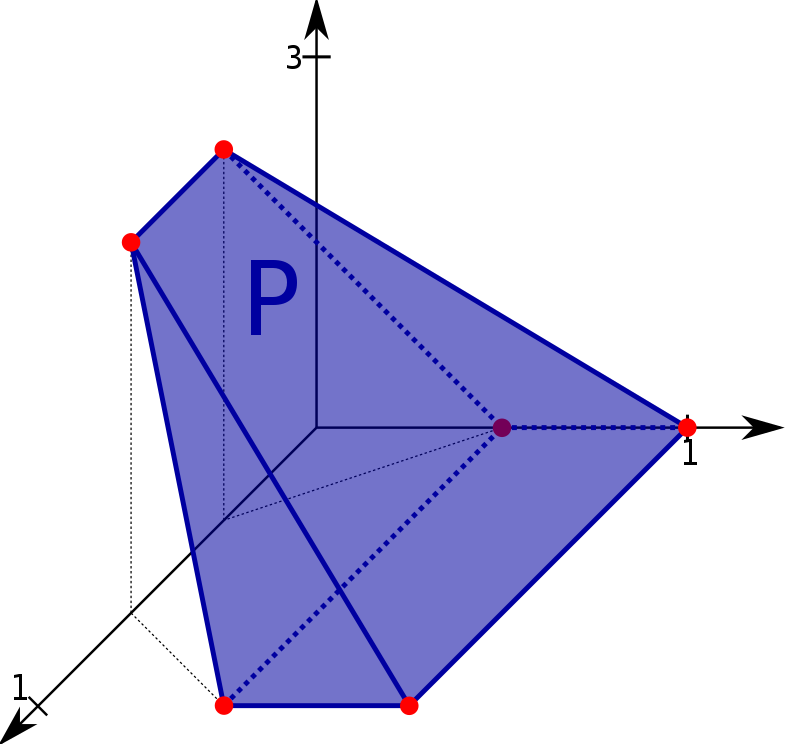
\includegraphics[width=0.7\textwidth]{region_factible_LP.png}
    \caption*{Una ilustración de una posible región factible en $\R^3$}
\end{figure}

Los bordes de la región factible están dados por los hiperplanos de la ecuación $Ax = b$. También es posible que la región no esté acotada: en cuyo caso puede pasar que el problema no tenga solución, y se pueda tomar valores de la función objetivo tan chicos como se desee.

\subsection{Método Simplex}

El \textit{método simplex} es un algoritmo para resolver problemas de programación lineal. Se basa en recorrer los vértices de la región factible (también llamada \textit{simplex}), ya que la solución óptima se debe encontrar en uno de ellos. En cada movimiento que realiza, la función objetivo no crece (e, idealmente, decrece). Como la cantidad de vértices crece exponencialmente con respecto a la cantidad de restricciones, el algoritmo es exponencial, y efectivamente corre lentamente para ciertos casos patológicos. No obstante, este algortimo es muy eficiente, y ampliamente utilizado, en la práctica.

\subsection{Reducciones}

Varios de los problemas de grafos que vimos en la materia se pueden reducir a programas lineales

\subsubsection{Flujo de costo mínimo}

Las restricciones de flujo de costo mínimo se dan en formato de programa lineal, así que la reducción es directa. Para una red de flujo $N = (V, E, u, b, c)$ Las ecuaciones e inecuaciones son:
\begin{gather*}
    \min{\sum_{vw \in E} c_{vw} x_{vw}} \\
    \begin{flalign*}
         &  & \sum_{w \in N^+(v)} x_{vw} - \sum_{w \in N^-(v)} x_{vw} & = b_v       &  & \forall v \in V  \\
         &  & x_{vw}                                                  & \geq l_{vw} &  & \forall vw \in E \\
         &  & x_{vw}                                                  & \leq u_{vw} &  & \forall vw \in E
    \end{flalign*}
\end{gather*}

\subsubsection{Flujo máximo}

Similarmente, se puede reducir el problema de flujo máximo a programación lineal\footnote{También se puede reducir ``pasando'' por flujo de costo mínimo, es decir, reducirlo primero a flujo de costo mínimo y luego a PL.}. Esto se logra de la siguiente manera:
\begin{gather*}
    \max{\sum_{v \in N^+(s)} x_{sv}} \\
    \begin{flalign*}
         &  & \sum_{w \in N^+(v)} x_{vw} - \sum_{w \in N^-(v)} x_{vw} & = 0         &  & \forall v \in V - \{s, t\} \\
         &  & x_{vw}                                                  & \geq 0      &  & \forall vw \in E           \\
         &  & x_{vw}                                                  & \leq u_{vw} &  & \forall vw \in E
    \end{flalign*}
\end{gather*}

\subsubsection{Camino mínimo}

Para un grafo pesado $V = (V, E, w)$ y un par de vértices $s, t \in V$, encontrar el camino mínimo entre $s$ y $t$ también se puede expresar como programa lineal, donde la variable $x_{uv}$ indica si una arista se utiliza ($x_{uv} = 1$) o no ($x_{uv} = 0$):
\begin{gather*}
    \max{\sum_{uv \in E} x_{uv} w_{uv}} \\
    \begin{flalign*}
         &  & \sum_{w \in N^-(t)} x_{vw}                              & = 1 &  &
         &  & \sum_{w \in N^+(v)} x_{vw} - \sum_{w \in N^-(v)} x_{vw} & = 0 &  & \forall v \in V - \{s, t\} \\
    \end{flalign*}
\end{gather*}

Esta reducción es equivalente a la reducción anterior de camino mínimo a flujo de costo mínimo. Las propiedades de la matriz de coeficientes garantizan que hay una solución óptima con $x_{ij} \in \{0, 1\}$.

\subsubsection{Árbol Generador Mínimo}

El problema de encontrar un AGM para un grafo pesado $G = (V, E, w)$ se puede expresar como el siguiente progama lineal:
\begin{gather*}
    \max{\sum_{uv \in E} x_{uv} w_{uv}} \\
    \begin{flalign*}
         &  & \sum_{uv \in E(S)} x_{vw} & \leq |S| - 1 &  & \forall S \subseteq V      \\
         &  & \sum_{uv \in E} x_{vw}    & = n - 1      &  & \forall v \in V - \{s, t\} \\
         &  & x_{vw}                    & \geq 0       &  & \forall vw \in E
    \end{flalign*}
\end{gather*}

También se puede demostrar que esta formulación tiene un óptimo entero. A pesar de que esta formulación tiene una cantidad exponencial de restricciones con respecto al tamaño del grafo original, se puede resolver en tiempo polinomial.

\subsection{P-Completitud}

No solo son los problemas anteriores los que se pueden reducir a PL: se puede demostrar que la programación lineal es P-Completo, esto es, cualquier problema resoluble en tiempo polinomial se puede reducir a él. En este sentido, es el problema ``más general'' entre ellos.

La teoría de clases de complejidad se estudia más en el \hyperref[capitulo-np-completitud]{siguiente capítulo}.

\subsection{Dualidad}

Para un problema de optimización que implica minimizar un valor, el \textit{problema dual} es uno que busca maximizarlo, y cuya solución es al menos tan grande como cualquier solución factible del primer problema (y viceversa para los problemas de maximización). Esto implica que si se encuentra una solución en la que coinciden, esta es mínima para el problema original.

Para la programación lineal, el problema dual de cualquier instancia es otro programa lineal. Si la instancia es:
$$\max{\{c^T x \mid x \in \R^n, Ax \leq b\}}$$

El programa lineal dual es:
$$\min{\{y^T b \mid y \in \R^m, y^T A \geq c\}}$$

\begin{theorem*}
    (Teorema de Dualidad Fuerte) Si un problema tiene una solución óptima, entonces el problema dual también la tiene, y sus valores coinciden.
\end{theorem*}


\chapter{NP-Completitud}
\label{capitulo-np-completitud}

\section{Problemas}

\subsection{Versiones}

Dada una instancia $I$ del problema de optimización $\Pi$ con función objetivo $f$, se pueden derivar varias versiones:
\begin{itemize}
    \item Versión de \textbf{optimización}: Encontrar una \underline{solución óptima} $S^*$ del problema $\Pi$ para $I$ (con $f(S^*) \geq f\ \forall S$ en el caso de maximización y $f(S^*) \le f\ \forall S$ para la minimización).
    \item Versión de \textbf{evaluación}: Determinar el \underline{valor} $f(S^*)$ de una solución óptima de $\Pi$ para $I$.
    \item Versión de \textbf{localización}: Dado un número $k$, determinar una solución factible $S$ de $\Pi$ para $I$ tal que \underline{$f(S) \leq k$} si el problema es de minimización, o $f(S) \geq k$ si es de maximización.
    \item Versión de \textbf{decisión}: Dado un número $k$, ¿\underline{Existe} una solución factible $S$ de $\Pi$ para $I$ tal que $f(S) \leq k$ si el problema es de minimización, o $f(S) \geq k$ si es de maximización?
\end{itemize}

Tomemos el ejemplo del problema de viajante de comercio:

\begin{problema}
    Dado un grafo pesado $G = (V, E, w)$, encontrar un \textit{circuito hamiltoniano} de peso mínimo, es decir, un circuito simple $C^*$ que pase por todos los vértices y minimice su peso total:
    $$C^* = \arg\min\left\{\sum_{e \in C} w(e) \mid C \text{ es circuito hamiltoniano en $G$}\right\}$$
\end{problema}

Para este problema, las versiones serían:
\begin{itemize}
    \item Versión de \textbf{optimización}: Encontrar un circuito hamiltoniano en $G$ de peso mínimo.
    \item Versión de \textbf{evaluación}: Determinar la longitud mínima que puede tener un circuito hamiltoniano en $G$.
    \item Versión de \textbf{localización}: Dado un número $k$, encontrar un circuito hamiltoniano en $G$ que tenga peso menor o igual a $k$.
    \item Versión de \textbf{decisión}: Dado un número $k$, ¿Existe un circuito hamiltoniano en $G$ que tenga peso menor o igual a $k$?
\end{itemize}

Para muchos problemas de optimización combinatoria, las cuatro versiones son equivalentes: si una de ellas puede resolverse eficientemente, las demás también. El estudio se realiza en la versión más simple: la de \underline{decisión} (y hay problemas que no tienen versión de optimización). Estos tienen dos respuestas posibles: \textbf{SÍ} o \textbf{NO}.

\subsection{Definición}

Un problema $\Pi$ se define dando su entrada y su salida:
\begin{problema}
    \textsc{Satisfactibilidad (SAT)}
    \medskip

    Dada una \textit{fórmula proposicional $f$} en forma normal conjuntiva, ¿Existe una asignación de valores de verdad ($\{True, False\}$) a las proposiciones de $f$ que hace que $f$ sea verdadera?
\end{problema}

Una \textit{instancia} $I$ de un problema es una especificación de sus parámetros. En el ejemplo de SAT, sería una fórmula CNF.

Un problema de decisión $\Pi$ tiene asociado un conjunto $I_{\Pi}$ de instancias, y un subconjunto de ellas $Y_{\Pi} \subseteq I_{\Pi}$ cuya respuesta es \textbf{SÍ}.

\section{Máquinas de Turing}

\subsection{Máquina de Turing Determinística}

Una \textit{máquina de Turing determinística} (MTD) es un modelo de cómputo simple. La máquina cuenta con:
\begin{itemize}
    \item Una \textit{cabeza lecto-escritora}, que se puede mover 1 unidad en ambas direcciones (Definido como $M = \{+1, -1\}$).
    \item Una \textit{cinta infinita} en ambas direcciones con celdas indexadas en $\Z$.
    \item Una celda inicial con índice $0$.
\end{itemize}

Esas son las características generales de cualquier MTD. Para una máquina particular, se tiene:
\begin{itemize}
    \item Un \textit{alfabeto} de \textit{símbolos} finito $\Sigma$ y un símbolo especial $\ast$ llamado ``\textit{blanco}''. Se define $\Gamma = \Sigma \cup \{\ast\}$. Las celdas puede tomar valores en $\Gamma$.
    \item Un conjunto finito $Q$ de \textit{estados}.
    \item Un \textit{estado inicial} $q_0 \in Q$.
    \item Un conjunto de \textit{estados finales} $Q_f \subseteq Q$ (en el caso de problemas de optimización $Q_f = \{q_{\text{sí}}, q_{\text{no}}\}$).
    \item Un \textit{programa}, definido como un conjunto finito de \textit{instrucciones}. Estas, a su vez, están definidas como quíntuplas $S \in Q \times \Gamma \times Q \times \Gamma \times M$, y una instrucción $(q, s, q', s', m)$ se interpreta como: ``Si la máquina está en el estado $q$ y la cabeza lee el símbolo $s$, entonces escribe $s'$ en esa celda, realiza el movimiento $m$, y pasa al estado $q'$''.
\end{itemize}

La entrada al programa se carga utilizando los símbolos de $\Sigma$, y las demás celdas en la cinta empiezan con el valor $\ast$.

El modelo es capaz de simular cualquier otra máquina Turing-equivalente, lo cual incluye a la \hyperref[maquina-ram]{máquina de RAM} analizada anteriormente.

\subsubsection{Determinismo}

Las MTDs son \textit{determinísticas}: para todo par $(q, s) \in Q \times \Gamma$, existe en el programa a lo sumo una quíntupla que comienza con ese prefijo. Esto implica que, en cada paso, no hay ambigüedad respecto a qué hacer (porque solo una instrucción aplica).

\subsubsection{Resolución y Complejidad}

La máquina \textit{resuelve} el problema $\Pi$ si para toda instancia $I \in I_{\Pi}$ esta alcanza un estado final y es el correcto.

La \textit{complejidad} de una MTD está dada por la cantidad de movimientos de la cabeza que se realizan entre el estado inicial y el final, en función del tamaño de entrada:
$$T_M(n) = \max\{m \mid M \text{ realiza $m$ movimientos para la entrada $I \in I_{\Pi}, |I| = n$}\}$$

Una MTD $M$ es \textit{polinomial} para $\Pi$ cuando $T_M(n) \in \BigO{n^k}$ para algún $k$.

\subsection{La clase P}

Un problema de decisión $\Pi$ pertenece a la clase P si existe una MTD polinomial que lo resuelve. Esto equivalente a que exista un algoritmo polinomial (en la máquina RAM) que resuelve $\Pi$. Hay problemas (como la \hyperref[programacion-lineal]{programación lineal}) que son P-completos: cualquier problema de P se puede reducir a una instancia de ellos

\subsection{Máquina de Turing no Determinística}

Una máquina de Turing no determinística (MTND) es una máquina de Turing en la que no se requiere unicidad para el prefijo $(q, s)$ con el que empieza cada instrucción. En el caso de estar en un estado y símbolo donde múltiples instrucciones aplican, la máquina elige cualquiera de ellas (no está especificado cuál).

\subsubsection{Resolución y Complejidad}

Una MTND resuelve el problema de decisión $\Pi$ cuando existe una secuencia de ejecución de instrucciones que lleva a un estado de aceptación si y solo si la respuesta correcta es sí. La ejecución se puede interpretar como un \textit{árbol de alternativas}, donde cada nodo representa un punto en el que se puede ``elegir'' entre 1 o más instrucciones válidas.

Una definición equivalente sería que para toda instancia de $Y_{\Pi}$ existe \textbf{al menos una} rama de ejecución que termina en $q_{\text{sí}}$, mientras que para toda instancia de $I_{\Pi} - Y_{\Pi}$, ninguna lo hace.

Por otro lado, la complejidad temporal deuna MTND $M$ se define como el máximo número de pasos que toma la rama de ejecución más corta en llegar a $q_{\text{sí}}$ para una instancia de $Y_{\Pi}$ en función de su tamaño:
$$T_M(n) = \max\{m \mid \text{La rama más corta de $M$ termina en $m$ movimientos para $x \in Y_{\Pi}, |x| = n$}\}$$

Una MTND $M$ es polinomial para $\Pi$ cuando $T_M(n) \in \BigO{n^k}$ para algún $k$.

\subsection{La clase NP}

Un problema de decisión $\Pi$ pertenece a la clase NP (polinomial no-detereminístico) cuando existe una MTND polinomial que lo resuelve.

Una definición equivalente es que, dada una instancia $I \in Y_{\Pi}$, se puede dar un \textit{certificado} de longitud polinomial (con respecto al tamaño de $I$) que garantiza que la respuesta es \textbf{SÍ}, y esto se puede verificar en tiempo polinomial.

Una observación es que $P \subseteq NP$: para un problema polinomial, una instancia $I \in Y_{\Pi}$ es su propio certificado, ya que tiene tamaño lineal con respecto a sí misma y se puede verificar aplicando el algoritmo que resuelve el problema que, por definición, es polinomial.

\begin{theorem*}
    Si $\Pi$ es un problema de decisión que pertenece a la clase NP, entonces $\Pi$ puede ser resuelto por un algoritmo determinístico en tiempo exponencial con respecto al tamaño de la entrada.
\end{theorem*}
\begin{proof}
    Para resolver $\Pi$, se puede simular la ejecución de la MTND que lo resuelve: cada vez que hay ambigüedad con respecto a la instrucción a aplicar se exploran todos los ``súbarboles de ejecución''. Esto implica una complejidad exponencial: si hay a lo sumo $A$ estados distintos para cada punto de no-determinismo, se realizan \BigO{A^{T_M(n)}}, y $T_M(n)$ es una función polinomial (porque $\Pi \in \text{NP}$).
\end{proof}

\subsubsection{P vs. NP}

El problema abierto más famoso en la ciencia de la computación es el de P vs. NP, esto es, es la clase P la misma que NP. Se sabe que $P \subseteq NP$, así que lo que se demostraría es si $NP \subseteq P$ o $NP \subsetneq P$. Si P fuera igual a NP, entonces cualquier problema que se pueda certificar en tiempo polinomial se podría resolver también en tiempo polinomial.

\subsection{Reducciones Polinomiales}
\label{reducciones}

Una \textit{transformación} o \textit{reducción polinomial} de un problema de decisión $\Pi'$ a otro $\Pi$ es una función $f: I_{\Pi'} \longrightarrow I_{\Pi}$ que puede ser computada en tiempo polinomial y cumple que:
$$I' \in Y_{\Pi'} \iff f(I') \in Y_{\Pi} \forall I' \in I_{\Pi'}$$

Es decir, una instancia de $\Pi'$ tiene respuesta sí si y solo si la instancia correspondiente $f(I')$ tiene respuesta sí.

Se dice que un problema de decisión $\Pi'$ se \textit{reduce polinomialmente} a otro $\Pi$ cuando existe una reducción polinomial entre $\Pi'$ y $\Pi$. Se denota $\Pi' \leq_p \Pi$.

Las reducciones polinomiales son \textbf{transitivas}: si $\Pi_1 \leq_p \Pi_2$ y $\Pi_2 \leq_p \Pi_3$ entonces $\Pi_1 \leq_p \Pi_3$. Esto es porque, si las reducciones correspondientes son $f_{12}$ y $f_{23}$, se puede construir una función $f_{13}(I) = f_{23}(f_{12}(I))$.

\subsection{La clase NP-completo}
\label{np-completo}
\label{np-hard}

Un problema de decisión $\Pi$ es \textit{NP-completo} cuando:
\begin{enumerate}
    \item $\Pi \in NP$
    \item $\forall \bar{\Pi} \in NP, \bar{\Pi} \leq_p \Pi$
\end{enumerate}

Si un problema cumple la condición $2$, se lo llama \textit{NP-difícil}.

\begin{theorem*}
    (Teorema de Cook-Levin) SAT es NP-Completo.
\end{theorem*}
\begin{proof}
    Sabemos que $\textsc{SAT} \in NP$: para certificar una instancia $f \in Y_{\textsc{SAT}}$, se puede tomar la asignación de valores de verdad a las proposiciones de $f$. Tanto el tamaño de este certificado como verificarlo (que implica evaluar la fórmula en con los valores) son lineales.

    Para ver que es NP-hard, tomemos un problema cualquiera $\Pi \in NP$. Como está en NP, hay una MTND que lo resuelve. Llamamos:
    \begin{itemize}
        \item $\Gamma = \Sigma \cup \{\ast\}$ a su alfabeto.
        \item $Q$ a su conjunto de estados.
        \item $s \in Q$ al estado inicial.
        \item $F \subseteq Q$ al conjunto de estados finales.
        \item $\Delta \subseteq Q \times \Gamma \times Q \times \Gamma \times M$ al conjunto de instrucciones.
    \end{itemize}

    Asumimos $M = \{+1, 0, -1\}$ (el cabezal se puede quedar quieto).

    Reducimos $\Pi$ a SAT de la siguiente manera: dado un input $I$ de $\Pi$, construimos una fórmula proposicional $f$ tal que $f$ es satisfactible si y solo si $I \in Y_{\Pi}$. Sea $p(n)$ la función de complejidad de la MTND. La fórmula contiene las siguientes propocisiones:
    \begin{itemize}
        \item $T_{ijk} \equiv $ ``la celda $i$ contiene el símbolo $j$ en el paso $k$ de la ejecución de la MTND''
        \item $H_{ik} \equiv $ ``el cabezal de la MTND está ubicado en la celda $i$ en el paso $k$''
        \item $Q_{qk} \equiv $ ``la MTND está en estado $q$ en el paso $k$''
    \end{itemize}

    Para $i = \{-p(n), ..., p(n)\}$ (el cabezal no se puede mover más que la cantidad máxima de pasos), $k = \{0, ..., p(n)\}$, $j \in \Gamma$ y $q \in Q$. Además, llamamos $I = (j_0, ..., j_{n - 1})$ a la entrada, que empieza en la celda $0$.

    Las cláusulas de la fórmula son las siguientes:
    \begin{itemize}
        \item $T_{i j_i 0}$: la celda $i$ contiene el valor $j_i$ en tiempo $0$, para $i = 0, ..., n - 1$.
        \item $T_{i \ast 0}$: la celda $i$ contiene el valor blanco en tiempo $0$, para $i \in \{-p(n), ..., p(n)\} - \{0, ..., n - 1\}$
        \item $H_{00}$: el cabezal comienza en la celda $0$.
        \item $Q_{s0}$: la máquina comienza en el estado $s$.
        \item $\neg (T_{ijk} \land T_{ij'k})$: la celda $i$ contiene a lo sumo un símbolo en el paso $k$ ($j \neq j'$).
        \item $\bigvee_{j \in \Gamma} T_{ijk}$: la celda $i$ contiene al menos un símbolo en el paso $k$.
        \item $T_{ijk} \land T_{ij'(k+1)} \implies H_{ik}$: las celdas no apuntadas por el cabezal no cambian ($j \neq j', k < p(n)$).
        \item $\neq (Q_{qk} \land Q_{q'k})$: la máquina está en a lo sumo un estado en el paso $k$ ($q \neq q'$).
        \item $\neq (H_{ik} \land H_{i'k})$: el cabezal apunta a lo sumo a una celda en el celda paso $k$ ($i \neq i'$).
        \item $H_{ik} \land Q_{qk} \land T_{i \sigma k} \implies \bigvee_{(q, \sigma, q', \sigma', m) \in \Delta} (H_{(i+m)(k + 1)} \land Q_{q'(k + 1)} \land T_{i \sigma (k + 1)})$: en cada paso $k < p(n)$, se da una de las transiciones válidas.
        \item $\bigvee_{k = 0}^{p(n)} \bigvee_{f \in F} Q_{fk}$: la máquina termina en un estado final.
    \end{itemize}

    Si hay un cómputo de la MTND con $I$ que termina en un estado $F$, entonces $f$ es satisfacible asignando las proposiciones correspondientes a la ejecución. Recíprocamente, si $f$ es satisfacible, entonces existe un cómputo de la MTND que, a partir de $I$ y siguiendo los pasos especificados por las proposiciones verdaderas, llega a un estado de $F$. Como la fórmula tiene \BigO{p(n)^2} proposiciones y \BigO{n^3} cláusulas, esta reducción es polinomial.

    Dado que esta reducción es posible para cualquier problema $\Pi \in NP$, SAT es NP-completo.
\end{proof}

Para demostrar la NP-completitud de otros problemas $\Pi' \in NP$, se puede reducir problemas conocidos NP-completos a ellos: si $\Pi$ es un problema NP-completo, entonces
$$\Pi \leq_p \Pi' \implies \forall \bar{\Pi} \in NP, \bar{\pi} \leq_p \Pi'$$

Esto vale por la transitividad de las reducciones polinomiales.

Para demostrar el caso $P = NP$, bastaría con encontrar un problema en $NP\text{-completo} \cap P$, ya que los demás problemas de NP podrían ser reducidos a ese problema y resueltos, todo en tiempo polinomial.

\section{Problemas NP-completos}

Como demuestra el teorema de Cook-Levin, SAT es NP-completo. Este hecho puede ser utilizado para demostrar la NP-completitud de múltiples problemas: en 1972, Karp demostró que otros 21 problemas son NP-completos. En la actualidad se conocen más de 3000 problemas problemas NP-completos.

\subsection{3-SAT}
\label{3-sat}

3-SAT es una versión restringida de SAT, donde las fórmulas CNF $f$ tienen exactamente 3 literales. A pesar de ser aparentemente menos general, este problema también es NP-completo.
\begin{theorem*}
    3-SAT es NP-completo
\end{theorem*}
\begin{proof}
    Para demostrar que está en NP, se puede tomar el mismo certificado y verificador que para SAT: la asignación de valores que hace a $f$ verdadera.

    Para demostrar que es NP-hard, se puede reducir SAT a 3-SAT. Esto se logra tomando cada cláusula $(p_{i1} \lor \cdots \lor p_{ik})$ y agregando distintas cláusulas dependiendo de su tamaño:
    \begin{itemize}
        \item Si $k = 1$, la cláusula tiene una sola proposición: $p_{i1}$. En ese caso se puede agregar el conjunto de cláusulas
              \begin{align*}
                  (p_{i1} \lor q_{i1} \lor q_{i2})\            & \land \\
                  (p_{i1} \lor \neg q_{i1} \lor q_{i2})\       & \land \\
                  (p_{i1} \lor q_{i1} \lor \neg q_{i2})\       & \land \\
                  (p_{i1} \lor \neg q_{i1} \lor \neg q_{i2})\  &
              \end{align*}

              Se puede ver que la única forma de que este grupo de cláusulas sea verdadero es que $p_{i1}$, ya que cualquier asignación de los parámetros $q_{i1}, q_{i2}$ hace que alguna de ellas sea falsa.

        \item Si $k = 2$, la cláusula tiene 2 proposiciones: $(p_{i1} \lor p_{i2})$. En su lugar, se agregan dos cláusulas:
              $$(p_{i1} \lor p_{i2} \lor q_i) \land (p_{i1} \lor p_{i2} \lor \neg q_i)$$

              Este par de cláusulas es verdadero si y solo si la cláusula original es verdadera: el valor de la variable $q_i$ no afecta esto.

        \item Si $k = 3$, se pone la misma cláusula en la fórmula.
        \item Si $k > 3$, se puede usar el siguiente conjunto de cláusulas:
              \begin{align*}
                          & (p_{i1} \lor p_{i2} \lor q_{i1})                  \\
                  \land\  & (\neg q_{i1} \lor p_{i3} \lor q_{i2})             \\
                          & \vdots                                            \\
                  \land\  & (\neg q_{i(j - 2)} \lor p_{ij} \lor q_{i(k - 1)}) \\
                          & \vdots                                            \\
                  \land\  & (\neg q_{i(k - 3)} \lor p_{i(k - 1)} \lor q_{ik})
              \end{align*}

              Este conjunto de cláusulas es verdadero si y solo si $(p_{i1} \lor \cdots \lor p_{ik})$ es verdadero.
    \end{itemize}

    Como cada componente de la nueva conjunción $f'$ es satisfactible si y solo si el término correspondiente de $f$ lo es, $f \iff f'$. Además, el tamaño de la nueva fórmula es a lo sumo 3\footnote{No estoy seguro} veces más grande que la anterior, así que la reducción es polinomial. Queda demostrado $3-\text{SAT} \leq_p \text{SAT}$.

\end{proof}

\subsection{Clique máxima}
\label{clique}

\begin{problema}
    \textsc{Clique}
    \medskip

    \textbf{Entrada}: Un grafo $G = (V, E)$

    \textbf{Salida}: Un subgrafo inducido completo (también llamado clique) $K_m \subseteq G$ tal que
    $$|K_m| \geq |S|\ \forall S \subseteq G, S \text{ es clique en } G$$
\end{problema}

La versión de decisión del problema de clique máxima es determinar si existe alguna clique en $G$ con tamaño mayor o igual $k$ para un $k$ dado.

\begin{theorem*}
    \textsc{Clique} es NP-completo
\end{theorem*}
\begin{proof}
    % TODO
\end{proof}

% TODO: Maximum independent set, coloreo

\section{Restricción y Extensión}

\subsection{Definición}

El problema $\Pi$ es una \textit{restricción} de otro problema $\bar{\Pi}$ si el dominio de $\Pi$ está incluido en el dominio de $\bar{\Pi}$, y la salida de ambos problemas es la misma (es decir, son el mismo problema, pero $\Pi$ tiene una entrada restringida). Cuando sucede esto, se dice que $\bar{\Pi}$ es una \textit{extensión} o \textit{generalización} de $\Pi$.

Es habitual que una restricción de un problema de NP-completo esté en P, pero que la situación recíproca no pueda suceder (a menos que P = NP).

\subsection{Ejemplos}

\begin{itemize}
    \item Como vimos en la \hyperref[3-sat]{sección anterior}, 3-SAT es una restricción de SAT, pero ambos problemas son NP-completos. Por otro lado, 2-SAT (también una restricción de SAT) es polinomial.
    \item Coloreo es un problema NP-completo, y lo sigue siendo para:
          \begin{itemize}
              \item Grafos arco-circulares.
              \item Grafos que no contienen a $P_5$ como subgrafo inducido.
              \item Grafos planares.
              \item Grafos sin triángulos.
          \end{itemize}

          Sin embargo, se vuelve polinomial si se restringe a:
          \begin{itemize}
              \item Grafos arco-circulares propios.
              \item Cografos (grafos sin $P_4$ inducido).
              \item Grafos de intervalos.
              \item Grafos cordales.
              \item Grafos perfectos.
              \item Grafos sin subgrafos inducidos $K_{1, 3}$.
          \end{itemize}

    \item $k$-\textsc{Clique}, una restricción de \textsc{Clique} en la cual el tamaño de la clique es fijo, es polinomial para cualquier $k$. Esto se debe a que se pueden ennumerar todas las combinaciones de vértices de tamaño $k$ en tiempo \BigO{n^k} (lo cual, para $k$ fijo, es polinomial) y verificar si son cliques en tiempo cuadrático. Esto funciona porque cualquier grafo que tiene una clique de tamaño mayor a $k$ tiene otra(s) de tamaño exactamente $k$ como subgrafo de esta. El resultado implica que el problema \textsc{Clique en grafos planares} es polinomial, porque los grafos planares no pueden tener a $K_5$ como subgrafo (así que se puede reducir a \textsc{4-Clique}).
\end{itemize}

\section{La clase co-NP}

\subsection{Problema complemento}

El \textit{problema complemento} de un problema de decisión $\Pi$, $\Pi^c$, es un problema de decisión con el mismo conjunto de instancias, pero cuya respuesta es \textbf{SÍ} para todas las instancias \textbf{NO} de $\Pi$, y viceversa. Es decir, $\Pi^c$ cumple:
\begin{itemize}
    \item $I_{\Pi^c} = I_{\Pi}$
    \item $Y_{\Pi^c} = I_{\Pi} - Y_{\Pi}$
\end{itemize}

Un ejemplo posible sería \textsc{Tautology}: Dada una fórmula $f$ en DNF, es $f$ una tautología. Esto es cierto si y solo si $\neg f$, una fórmula CNF, es una contradicción, es decir, no se puede satisfacer, así que el problema responde \textbf{SÍ} para las instancias de \textsc{SAT} que no son satisfactibles.

\begin{theorem*}
    Si un problema $\Pi$ está en $P$, entonces $\Pi^c \in P$.
\end{theorem*}
\begin{proof}
    Si existe un algoritmo polinomial para resolver $\Pi$ en tiempo polinomial, la respuesta de ese algoritmo se puede invertir, obteniendo un algoritmo polinomial para $\Pi^c$.
\end{proof}

Este argumento no sirve para la clase NP: que $\Pi$ esté en NP significa que hay un certificado y verificador polinomiales para las instancias de $Y_{\Pi}$ (no necesariamente para las de $Y_{\Pi^c} = I_{\Pi} - Y_{\Pi}$).

\subsection{co-NP}

La clase co-NP está definida como aquellos problemas cuyo complemento está en NP, es decir:
$$\Pi \in NP \iff \Pi^c \in co-NP$$

Una definición alternativa sería que son aquellos problemas donde existen certificado y verificador polinomiales para instancias de respuesta \textbf{NO}. El problema \textsc{Tautology}, mencionado anteriormente, es un ejemplo de un miembro de esa clase y, más aún, es co-NP-completo: cualquier problema de co-NP se puede reducir polinomialmente a este.

\begin{theorem*}
    Si $\Pi \in$ NP-completo, $\Pi^c \in$ co-NP-completo
\end{theorem*}
\begin{proof}
    Si $\Pi$ es NP-completo existe, para cualquier problema $\bar{\Pi} \in$ NP, una reducción polinomial a $\Pi$. Esta misma reducción se puede aplicar entre problemas de co-NP y $\Pi^c$.
\end{proof}


\end{document}
